% \documentclass[11pt]{article}
\documentclass[review,hidelinks,onefignum,onetabnum]{siamart220329}

% Packages and macros go here
\usepackage{bbm}
\usepackage{subcaption}
\usepackage{amssymb}

\newcommand{\e}{\mathrm{e}}
\newcommand{\pder}[2]{\frac{\partial #1}{\partial #2}}
\newcommand{\R}{\mathbb{R}}
\newcommand{\C}{\mathbb{C}}
\newcommand{\N}{\mathbb{N}}
\newcommand{\bn}{\mathbf{n}}
\newcommand{\bx}{\mathbf{x}}
\newcommand{\bz}{\mathbf{z}}
\newcommand{\btau}{\boldsymbol{\tau}}
\newcommand{\bhx}{{\mathbf{\hat{x}}}}
\newcommand{\bhy}{\mathbf{\hat{y}}}
\newcommand{\hx}{{\hat{x}}}
\newcommand{\hy}{{\hat{y}}}
\newcommand{\hvarphi}{{\hat{\varphi}}}
\newcommand{\hPhi}{{\hat{\Phi}}}
\newcommand{\by}{\mathbf{y}}
\newcommand{\br}{\boldsymbol{r}}
\newcommand{\btheta}{\mathbf{\theta}}
\newcommand{\de}{\,\mathrm{d}}
\newcommand{\htau}{{\hat{\tau}}}
\newcommand{\hpsi}{{\hat{\psi}}}
\newcommand{\M}{\mathcal{T}}
\newcommand{\surface}{\Gamma_{f}}
\newcommand{\solid}{\Gamma_{s}}
\newcommand{\tvarphi}{\widetilde \varphi}
\newcommand{\real}{\operatorname{Re}}
\newcommand{\imag}{\operatorname{Im}}

\newsiamthm{remark}{Remark}

\DeclareMathOperator{\sign}{sign}

% \topmargin -.5in
% \oddsidemargin 0pt
% \textheight 8.8in
% \textwidth 6.5in

\title{Complex-scaled boundary integral equation for time-harmonic water waves}

\author{Anne-Sophie Bonnet-Bendhia\thanks{POEMS, CNRS, Inria, ENSTA Paris, Institut Polytechnique de Paris,  France.}
\and Luiz M. Faria\footnotemark[1]
\and Carlos Perez-Arancibia\thanks{Department of Applied Mathematics, University
of Twente, Enschede,  The Netherlands}
}

\graphicspath {{../figures/}}

\date{\today}

\begin{document}

\maketitle

% REQUIRED
\begin{abstract}  
  We present a novel boundary integral equation (BIE) formulation for the
  time-harmonic water-waves problem based on a complex-scaled Laplace's
  free-space Green's function. The method makes use of a perfectly matched layer
  (PML) coordinate stretching to render propagating waves exponentially
  decaying, allowing for the efficient truncation of the unbounded free surface and bottom topography. We focus here on a two-dimensional 
 formulation which uses only simple function evaluations (e.g. complex logarithms
  and square roots), avoiding the need to compute the water-wave Green's
  function. We show through a variety of numerical examples that, despite the logarithmic growth of the complex-scaled Laplace's
  free-space Green's function, the truncation
  errors are exponentially small with respect to the truncation length. This approach can also be used to compute complex resonances through a \emph{linear} eigenvalue problem since the Green's function is frequency-independent. 
\end{abstract}

% REQUIRED
\begin{keywords}
    Water waves, finite depth, perfectly matched layers, boundary integral equations, Nystr\"om method. 
\end{keywords}

%\noindent \textbf{AMS subject classifications}:

% \tableofcontents

\section{Introduction}

Wave propagation and scattering problems in physics and engineering often involve unbounded domains that include infinite boundaries. These types of models are particularly important in various scenarios, such as seismic waves interacting with the free surface, outdoor sound propagation, guided (acoustic, electromagnetic, elastic) wave phenomena, and water waves propagating at the ocean's free surface, to mention a few. This paper specifically focuses on the linear (finite-depth) time-harmonic water wave problem, which features two infinite boundaries modeling the bottom topography and the free surface. 
This classical problem can be traced back to the work of Cauchy~\cite{cauchy1816theory} and originated from the study of the hydrodynamics of floating and submerged bodies. The simple model considered in this paper could serve as a prototypical example for investigating a wide range of simplified wave problems where the oscillations of volumetric waves can be neglected at the scale of surface waves. This is typically the case in plasmonics, where the relevant physical phenomenon is the presence of (subwavelength) surface plasmon polaritons~\cite{maier2007plasmonics}.

%This classical problem, which can be traced back to the work of Cauchy~\cite{cauchy1816theory} and originated from the study of the hydrodynamics of floating and submerged bodies, may also find applications in other fields such as plasmonics, where surface plasmon polaritons~\cite{maier2007plasmonics}, and seismology, where Rayleigh and Love waves~\cite{graff2012wave}, are important. Indeed, the simple linear water wave model considered in this paper serves as a prototypical example for investigating a wide range of simplified wave problems where the oscillations of volumetric waves can be neglected at the scale of surface waves, while high-frequency surface waves remain significant.

While boundary integral equation (BIE) methods are well known for their effectiveness in handling unbounded domains, they encounter notable challenges when applied to problems involving infinite boundaries. BIEs naively formulated using free-space Green's functions over the entire domain inherently result in equations defined on the domain's infinite boundaries. Therefore, suitable truncation techniques become essential to enable their numerical solution, provided, of course,  sufficient decay of the integrands exists. The simple approach of abruptly truncating the computational domain at some distance far from the wave sources offers limited success in the case of the Helmholtz equation due to the slow decay of the free-space Green's function, and becomes completely ineffective when applied to two-dimensional water wave problems due to the logarithmic growth of Laplace's free-space Green's function. We mention in passing, that  a domain decomposition approach that uses the free-space Green's function together with a BIE formulation over a bounded domain, has been pursued in \cite{mei1978numerical,yeung1982numerical}. In those works, a Dirichlet-to-Neumann map based on a modal series expansion of the scattered velocity potential is used to effectively reduce the problem to a bounded domain, an idea that later seemed to have influenced the development of finite element methods for water wave problems~\cite{lenoir1988localized}.

Leveraging the geometric simplicity of the infinite boundaries involved, many BIE formulations for water wave problems rely instead on the use of problem-specific Green's functions that exactly fulfill the relevant boundary conditions over infinite flat portions of the domain's boundaries~\cite{angell1991recent,angell1986integral,black1975wave,chakrabarti2001application,fenton1978wave,mackay2021green}. While these formulations yield BIEs posed on a bounded portion of the domain's boundary, the numerical evaluation of the associated Green's function often becomes the major bottleneck in the solution process since simple expressions for the free-surface Green's function are in general not available. Intricate numerical procedures have been developed in order to compute the free-surface Green's function (see e.g.~\cite{xie2018comparison} and~\cite{mackay2021green} for a comparison of  different techniques and recent developments on this subject). This evaluation typically entails  Fourier-like integrals, non-standard special functions, and/or power series expansions, which in view of the large number of function evaluations needed, can be computationally demanding~\cite{newman1985algorithms}. Furthermore, off-the-shelf acceleration techniques for the Laplace equation, such as the fast multipole method (FMM)~\cite{greengard1987fast}, cannot be directly applied to the free-surface Green's function. Interestingly, an explicit closed-form expression (in terms of exponential integrals) for the infinite depth problem in two dimensions, is presented in~\cite{hein2010explicit}. Even in this relatively simple case, developing a multipole expansion is non-trivial~\cite{perez2012fast}. Unfortunately, as far as the authors are aware, there are no closed-form expressions (nor multipole expansions) available for the two-dimensional finite depth problem as well as for the three-dimensional finite and infinite depth problems. We refer the reader to~\cite{martin2006multiple,hoernig2010green,linton2001mathematical} where these topics are discussed in great detail. In addition to the aforementioned efficiency issues, it is important to mention that problem-specific Green's functions always incorporate image sources which are essential for enforcing the free-surface and Neumann boundary conditions at flat boundaries. Their presence, however, imposes significant constraints on the types of domains where the associated BIE formulation can be applied. In fact, domains suitable for the application of such BIE formulations must be strictly confined within the strip defined by the flat free surface and the flat bottom topography.

Over the last decade, there have been notable advancements in the development of novel BIE formulations for Helmholtz wave problems involving unbounded interfaces~\cite{bruno2016windowed,lu2018perfectly}. These formulations revisit the idea of utilizing the simple efficient-to-evaluate free-space Green's function and truncating the resulting BIE posed on infinite boundaries, but they incorporate mechanisms to effectively account for the correct ``outgoing" solution behavior outside the bounded region of interest. In detail,~\cite{bruno2016windowed} puts forth the so-called Windowed Green's function (WGF) method, which features a real-valued suitably-scaled smooth window function that multiplies the free-space Green's function kernel to effectively reduce the BIE to a bounded domain. In essence, this method exploits the fact that windowed integrands exhibiting decaying and oscillatory behavior can be neglected from the tails of the integrals over the infinite boundaries, introducing errors that decay super-algebraically fast as the size of the truncated region increases. Around the same time, a technique was introduced by Lu et al. in~\cite{lu2018perfectly} that utilizes a BIE formulation of the PDE boundary value problem transformed by a perfectly matched layer (PML) complex stretching and subsequently truncated to a bounded domain. As the WGF method, the resulting PML-BIE formulation is posed on a bounded portion of the infinite boundary and features a modified free-space Green's function that encodes the outgoing oscillatory character of the PDE solution. 

Although the WGF proves effective at solving Helmholtz problems in the context of layered and periodic media as well as waveguides~\cite{bruno2016windowed,bruno2017windowed2,bruno2017windowed,strauszer2023windowed}, its direct application to the water wave problem under consideration is not feasible. While it may be tempting to attribute the failure of the WGF method to the logarithmic growth of the free space Green's function, an argument can be made that by combining an easy-to-evaluate harmonic function with the free-space Green's function, a decaying Green's function can be formed (in a manner akin to the construction used in~\cite{chandler1998uniqueness}). However, even in that scenario, it is easy to see that the WGF method would fail to approximate the correct radiative water wave problem solution.  Indeed, when considering real boundary data, the WGF method produces a real-valued (stationary-wave) solution that fails to approximate the correct radiative water wave problem solutions. We suspect that the failure of the WGF method in the context of the water waves problem is due to the fact that, unlike in the Helmholtz case, the Laplace free space Green's function contains no information about the ``correct`` radiation condition.

% an argument can be made that by combining an easy-to-evaluate harmonic function with the free-space Green's function, a decaying Green's function could be formed (in a manner akin to the construction used in~\cite{}), enabling then the application of the WGF method. However, even in that scenario, it is easy to see that the WGF method would fail to approximate the correct radiative water wave problem solution. \textcolor{red}{AS: We could say : this can be linked to the fact that when using the Windowed Green's function for Helmholtz, the size of the support of the window increases with the wavelength, and the tends to infinity when the frequency tends to zero. Or too difficult ?}

Building upon the PML-BIE method for the Helmholtz equation~\cite{lu2018perfectly}, this paper proposes a complex-scaled BIE method for the time-harmonic water wave problem in two dimensions. Our BIE formulation is derived from a direct integral representation of the analytically extended scattered velocity potential, obtained by suitably stretching the unbounded domain in the complex plane. This representation involves integrals over the infinite boundaries corresponding to the free surface and the bottom, and is obtained by applying  Green's third identity to the velocity potential and the logarithmic free-space Green's function over the complex stretched domain. Interestingly, despite the unboundedness of Laplace's Green's function along the complex stretched infinite boundaries, the resulting integral representation formula remains meaningful due to the provable exponential decay of the complexified velocity potential. Indeed, this decay is achieved by devising complex stretching coordinates on which the modal decomposition of the far-field scattered velocity potential, which encompasses a (constant-amplitude) propagating surface-wave mode and infinitely many evanescent modes, decays exponentially fast. Upon enforcing the boundary conditions and truncating the infinite boundaries, we then obtain a BIE that we solve numerically via a high-order Nystr\"om method which suitably handles the complexified kernels. Through our numerical experiments, we demonstrate that the error in the computed solutions using this methodology decays exponentially as the length of the PML region increases. 

A noteworthy difference with the PML-BIE technique applied to the Helmholtz equation~\cite{lu2018perfectly} stems from the fact that, due to the lack of wave-like behavior in the fundamental solution of Laplace's equation, its complex extension still exhibits a logarithmic growth at infinity (a more detailed discussion is given in~\Cref{sec:complex-scaled-formulation}). This makes it not immediately obvious that truncation errors stemming from the method will converge to zero as the length of the PML region is increased. While for the exact solution it is straightforward to show that the truncation of the involved integral operators to a bounded domain yields exponentially small errors (for the analytic extension of the exact solution decays exponentially at infinity), proving a stability result on the proposed truncation technique remains an open question. The main difficulty lies in the fact that the kernels in the proposed integral equation do not decay exponentially at infinity (in fact they may even grow logarithmically in some cases), and thus the integral operators over the unbounded curves are only well-defined for densities decaying sufficiently fast. The numerical results of~\Cref{sec:numerical-results} suggest, however, that the lack of decay in the Green's function is not a fundamental problem in the method, and much like in the Helmholtz case we observe truncation errors that decay exponentially fast as the length of the PML layer is increased.

To further showcase the capabilities and possible advantages of the proposed methodology, we numerically investigate the challenging problem of the scattering of a surface wave by an infinite step bottom topography, where a direct application of a BIE formulation that makes use of the problem-specific Green's function (satisfying free-surface and Neumann boundary conditions at the flat infinite boundaries), is not feasible. This limitation arises because the resulting integral equation becomes posed over a semi-infinite boundary~\cite{athanassoulis1999consistent,belibassakis2004three}. Finally, we apply our methodology to approximate the resonant frequencies that arise in floating body problems~\cite{Haz-Len-1993,mciver1996example}. In contrast to alternative approaches for computing complex resonances based on the use of the water-waves Green's function, which yields a (non-linear) eigenvalue problem where the frequency appears in the kernels of the integral operators~\cite{Haz-Len-1993}, our PML-transformed formulation gives rise to a linear (generalized) eigenvalue problem that can be efficiently solved using standard matrix eigenvalue solvers.

The paper is organized as follows. In~\Cref{sec:prob_setup} we provide the setup of the problem under consideration, recalling some standard results of water-waves theory. \Cref{sec:complex-scaled-formulation} focuses on the construction of the complex stretching based on the modal decomposition of the scattered velocity potential. The complex-scaled BIE formulation is then derived in~\Cref{sec:complex-scaled-bie}. In~\Cref{sec:Nyst_meth}, we introduce the Nystr\"om method employed in our approach. Next,~\Cref{sec:numerical-results} presents a variety of numerical experiments designed to validate the proposed methodology and also demonstrate its practical applicability. Finally, we present in~\Cref{sec:conclusions} some concluding remarks and possible future directions. 

% However, interestingly, the water wave problem presents novel theoretical and numerical challenges not present in Helmholtz-like problems. Mainly, such challenges have to do with the fact that Laplace's free-space Green's function is non-oscillatory, and as such its analytic extension does not become exponentially decaying inside the PML region. Despite the non-oscillatory behavior of the Laplace fundamental solution, which in fact grows logarithmically at infinity in two dimensions, we will argue that the solution can be analytically extended into the complex plane to become exponentially decreasing, justifying at least formally the truncation of certain integrals over unbounded domains. 

%While the WGF and PML-BIE methods both exhibit high-order convergence,  with the former exhibiting superalgebraic convergence and the latter exhibiting exponential convergence, there is a notable distinction in terms of implementation simplicity. The WGF method offers a significant advantage in this regard, as the modified Green's function can be obtained by straightforwardly multiplying the free-space Helmholtz Green's function by the window function. 
%Merely relying on the (slow) decay of the Green's function at infinity for a simplistic truncation of the BIE domain unavoidably leads to significant inaccuracies. 


% They recast the original PDE boundary value problem as a problem defined solely on the relevant boundaries of the domain. Upon discretization via e.g. Nystr\"om or boundary element methods, this approach leads to reduced-size linear systems that although dense can be made amenable to acceleration techniques such as the fast multipole method and H-matrices hence achieving nearly linear computational complexity. 
% %Moreover, unlike finite difference and finite element methods, BIE methods possess the advantage of seamlessly handling radiation conditions at infinity without the need for absorbing or transparent boundary conditions. Additionally, they yield PDE solutions that are free from numerical dispersion errors.
% While BIE methods offer significant advantages, 


% Solving such problem with a Boundary Element method set on the boundary of the scatterers requires the computation for each of these problems of a specific Green function, satisfying the right boundary condition on the straight infinite boundaries. This may be cumbersome, generally requiring the numerical evaluation of challenging integrals, and prevents of using existing tools for fast BEM like FMM which are conceived for simple free-space Green functions. (reference : Fast multipole boundary element method for the Laplace equation in a locally perturbed half-plane with a Robin boundary condition Carlos Pérez-Arancibia, Pedro Ramaciotti, Ricardo Hein, Mario Durán)

% An alternative to volume discretization methods are boundary integral equation
% methods, which rely on the use of a Green function to recast the PDE in terms of
% integral operators over the interfaces where the medium changes property. For
% piece-wise homogeneous media, this reduces the PDE to integral equations posed
% at the interface between the different media. Because boundary integral methods
% represent the solution as a sum of fundamental solutions which satisfy the
% radiation boundary condition, no domain truncation technique is required when
% the interfaces are bounded. This is a well-known advantage of boundary integral
% methods for scattering problems. There are interesting cases, however, where
% such interfaces are better modeled as infinite. Examples include the scattering
% of an object near the ground, the propagation of elastic waves under the surface
% of the earth, waveguides, and the water-waves problem described below. In such
% cases a truncation technique is required, at least in the direction parallel to
% the infinite interfaces, to reduce the problem to a finite subdomain where the
% equations can be discretized.


% This paper aims at the . While the WGF method offers some advantages when tackling layered media Helmholtz scattering problems, it fails at the produceing correct solutions of the water wave problems. As we will see in Section xxx, it is possible to construc a water wave problem with a real boundary data. The direct used othe WGF with the Laplace logartihmic kernel however, yields a real-valued stationary-like wave solution that does not exhibit the right outgoing behavior. 

% Another option is to use the simple free-space Green function and derive an integral equation on an infinite boundary. The price to pay is now to justify the new integral equation and, for  numerical purpose, to truncate the integral set on the unbounded surface, in such a way that the resulting error is as small as possible. This has been studied by several authors in the case of transmission problems for  the Helmholtz equation. It is worth mentioning that the naive approach of simply truncating the domain far enough from the region of interest is rather unsatisfactory. A very efficient solution, both accurate and easy to implement, is the so-called Windowed-Green function: thanks to a smooth truncation, the error due to the truncation is proved to decay super-algebraically. (references : Carlos, Oscar Bruno etc...)

% Let us notice  that the behavior of the solution at infinity, along the infinite boundary, is given by the behavior of the specific Green function but is in general completely different from that of the free-space Green function.  For instance, let us consider the 2D Helmholtz equation in a half-space with an impedance boundary condition so that a surface guided wave exists. In that case, the solution does not decay in general along the boundary, while the free-space Green function decays like $r^{-1/2}$. On the contrary, in the simple case of a Dirichlet boundary condition, the solution decays like  $r^{-3/2}$ along the boundary, so faster than the free-space Green function. This explains the difficulty in proving that the new integral equation provides the right ``outgoing'' solution of the scattering problem. More generally, the theory for this approach is still incomplete, but the numerical results are very convincing. 



% These type of problems pose significant challenges from both a theoretical and numerical point of view. Theoretically, one is required to impose appropriate conditions at infinity to
% guarantee the well-posedeness and the phyisical correctness of the partical differential equation (PDE) solutions. The numerical
% challenges, on the other hand, stem from the fact that the discretization scheme
% should incorporate information about the boundary conditions at infinity, also
% called radiation condition; this can be done directly, by e.g. expanding the
% solution in a basis which satisfy the radiation condition, or indirectly by
% truncating the domain to a finite size and imposing instead a carefully chosen
% boundary condition on the artificial boundaries of the truncated domain.


% Solving partial differential equations (PDEs) on unbounded domains poses
% additional challenges from both a theoretical and numerical point of view.
% Theoretically, one is required to impose appropriate conditions at infinity to
% guarantee uniqueness of solutions; when the underlying PDE comes from the
% modeling of the physical world, additional care must be taken to also ensure the
% recovered solution is the ``physically relevant'' one. The numerical
% challenges, on the other hand, stem from the fact that the discretization scheme
% should incorporate information about the boundary conditions at infinity, also
% called radiation condition; this can be done directly, by e.g. expanding the
% solution in a basis which satisfy the radiation condition, or indirectly by
% truncating the domain to a finite size and imposing instead a carefully chosen
% boundary condition on the artificial boundaries of the truncated domain.

% In the case of volume discretization methods such as finite difference and
% finite elements, a particular class of truncation techniques which enjoys great
% popularity due to its accuracy and simplicity is the Perfectly Matched Layers
% (PMLs) method. Loosely speaking, the method consists of solving for the analytic
% extension of the sought solution which decays exponentially at infinity. The
% decay rate of the analytic extension then facilitates the truncation of the
% domain upon discretization. On the physical (i.e. real) domain, PMLs can be
% reinterpreted as surrounding the computational region by a material layer, not
% necessarily physical, which absorbs but does not reflect incoming waves. A key
% difference between PMLs and \emph{ad hoc} absorbing material methods stem from
% the fact that the PML absorbing material is ``perfect'' in the sense that it is
% reflectionless at the continuous level (i.e. before discretization).


% In order to handle infinite interfaces in a boundary integral equation context,
% a few options are available. For relatively simple geometries and boundary
% conditions, one can construct a problem-specific Greens function which
% incorporates the boundary condition on all but a bounded portion of the
% interface, thus reducing the problem again to integrals over bounded
% curves/surfaces. This has the advantage of being conceptually simple provided
% such problem-specific Greens function can be efficiently computed.
% Unfortunately, for all but the simplest geometries, the representation of the
% problem-specific Greens function involves challenging integrals which must be
% approximated numerically. Alternatives that rely instead on the use of the
% free-space Greens function, readily available for many PDEs of physical
% relevance, have also been developed. In \cite{perez2017windowed} a high-order
% method called the Windowed-Green function (WGF) was introduced in order to
% truncate the integrals stemming from the boundary integral representation of the
% unbounded interfaces in the context of two- and three-dimensional
% Helmholtz/Maxwell scattering problems. At a similar time, \cite{lu2018perfectly}
% proposed a technique based on combining perfectly matched layers and a boundary
% integral representation on a certain truncated domain in the context of
% two-dimensional Helmholtz scattering problems. 
% % Due to the exponential decay of the Helmholtz Green function on the
% % complex-scaled PML layer, the kernels of the integral operators over the
% % infinite interfaces become exponentially small, allowing for an efficient
% % truncation with errors that decay exponentially respect to a truncation
% % parameter $\ell$ controlling the PML length. 
% It is worth mentioning the naive approach of simply truncating the domain far
% enough from the region of interest is rather unsatisfactory, especially for
% non-dissipative PDEs, due to the slow (algebraic) decay of the Greens function;
% in fact, as we will argue in this paper, such an abrupt truncation may not even
% converge in the zero-frequency regime, wherein the free-space Green function is
% no longer decaying.

% -- Window Green function does not work for water wave problems. Wangtao PML's paper. 
% -- Plasmonic applications 



% In this paper we build on the work of~\cite{lu2018perfectly} to develop a
% complex-scaled boundary integral equation method for the classical harmonic
% water-waves problem. The water-waves problem presents some interesting and novel
% challenges, of both theoretical and numerical nature, which are related to the
% fact that the free-space Green function is non-oscillatory, and as such its
% analytic extension does not become exponentially small inside the PML region
% (this contrasts the work in~\cite{lu2018perfectly}, where the exponential decay
% of the Helmholtz free-space Green's function facilitates the analysis). Despite
% the non-oscillatory behavior of the Laplace fundamental solution, which in fact
% grows logarithmically at infinity in two-dimensions, we will argue that the
% solution can be analytically extended into the complex plane to become
% exponentially decreasing, justifying at least formally the truncation of certain
% integrals over unbounded domains. 


\section{Problem setup}\label{sec:prob_setup}

We focus on linear and time-harmonic water waves in a bath of finite depth $d$. We present only the dimensionless equations, using the depth $d$ as a characteristic length scale (this means, in particular, that the dimensionless depth is one). 

Throughout this paper, we let $\Omega_f \subset \mathbb{R}^2$ denote the infinite fluid domain bounded above by the free surface $\Gamma_s$ and below by a bottom topography $\Gamma_b$. We also let $\Omega_o \subset \mathbb{R}^2$
denote the domain possibly occupied by bounded solid obstacles (either fully or partially) immersed in the fluid, with the immersed part of their boundary denoted by $\Gamma_o:=\partial \Omega_o\cap\overline\Omega_f$. More precisely, the free surface is assumed to be placed at $\R\times\{0\}$ so that $\Gamma_f = \R \times \{0\} \setminus
\overline\Omega_o$.  The bottom topography, on the other hand, is assumed to be given by a constant depth $1$ outside of a bounded domain, i.e., there exists an $L_0>0$ such that $\{|x_1|>L_0\}\times \{-1\}\subset\Gamma_b$. In the derivations that follow we use $L_1>\max\{L_0,\operatorname{diam}\Omega_o\}$. %Then, for $|x_1| > L$ the domain is a waveguide of constant depth. 
A schematic of the geometry is shown in~\Cref{fig:schematic-geometry}.

Here we seek to solve the following boundary value problem:
%
\begin{subequations}
  \label{eq:water-waves-system}
  \begin{align}  
    \Delta \varphi(\bx) &=0,\phantom{(\bx)} \quad\ \bx:=(x_1,x_2) \in \Omega:=\Omega_f\setminus\overline\Omega_o,\\
    \nabla \varphi(\bx) \cdot \bn(\bx) + \nu \varphi(\bx)&=f_1(\bx), \quad \bx \in \Gamma_f:=\Gamma_s\setminus\overline\Omega_o,\label{eq:impedance_bc}\\
    \nabla \varphi(\bx) \cdot \bn(\bx) &=f_2(\bx), \quad \bx \in \Gamma_b \cup \Gamma_o,\\
    \label{eq:radiation-condition}  
    \lim_{x_1 \to \pm \infty} \partial_{x_1} \varphi(\bx) \mp i k \varphi(\bx)  &= 0,
  \end{align}
\end{subequations}
%
where letting $\omega>0$ denote the angular frequency and $g$ the
gravitational acceleration, the term $\nu = (\omega^2d)/g$ in~\eqref{eq:impedance_bc} is an impedance-like dimensionless parameter, while the constant $k > 0$ in the radiation condition~\cref{eq:radiation-condition} is uniquely determined by the dispersion relation
\begin{align}
\label{eq:dispersion-relation}
k\tanh(k) = \nu.
\end{align}
%
As usual, $\bn\in\R^2$ is the unit normal which points toward the interior of the
fluid domain $\Omega$ (see~\Cref{fig:schematic-geometry}).  The unknown velocity potential $\varphi$ is  related to
the fluid velocity $\boldsymbol{u}$ through $\boldsymbol{u}(\bx,t) = \operatorname{Re}
\left(e^{-i\omega t} \nabla \varphi \right)$, where~$t$ is the time variable.

% In what follows we will non-dimensionalize~\cref{eq:water-waves-system-dimensional} using $d$ as a length scale and $\omega^{-1}$ as a temporal scale. Transforming $\bx \to d \bx$, $\varphi \to (d^2 \omega)\varphi$, the dimensionless equations become
% %
% \begin{subequations}
%   \label{eq:water-waves-system}
%   \begin{align}  
%     \label{eq:laplace-equation}
%     \Delta \varphi(\bx) &=0,\phantom{(\bx)} \quad\ \bx:=(x_1,x_2) \in \Omega:=\Omega_f\setminus\overline\Omega_o,\\
%     \label{eq:free-surface-bc}
%     \nabla \varphi(\bx) \cdot \bn(\bx) + \alpha^2 \varphi(\bx)&=f_1(\bx), \quad \bx \in \Gamma_f:=\Gamma_s\setminus\overline\Omega_o,\\
%     \label{eq:solid-bc}  
%     \nabla \varphi(\bx) \cdot \bn(\bx) &=f_2(\bx), \quad \bx \in \Gamma_b \cup \Gamma_o,\\
%     \label{eq:radiation-condition}  
%     \lim_{x_1 \to \pm \infty} \partial_{x_1} \varphi(\bx) \mp i k \varphi(\bx)  &= 0,
%   \end{align}
% \end{subequations}
% %
% where $\alpha = \omega \sqrt{d/g}$, $f_1 = 1/(\omega d) \hat{f}_1$, $f_2 = 1/(\omega d^2) \hat{f}_2$, and geometry has been properly adimensionalized. 

We here assume that the boundary data $f_1$ and $f_2$ are (compactly) supported in $\Gamma_f$ and $\Gamma_b$ vanishing over $\{|x_1|>L_2\}\times\{0\}$ and $\{|x_1|>L_2\}\times\{-1\}$, respectively. Note that the step-like bottom topography problem considered in~\Cref{sec:numerical-results} is not covered by the previous description; nevertheless, a slight modification of the assumptions made here allows us to extend the proposed PML-BIE approach to this challenging problem.

\begin{figure}
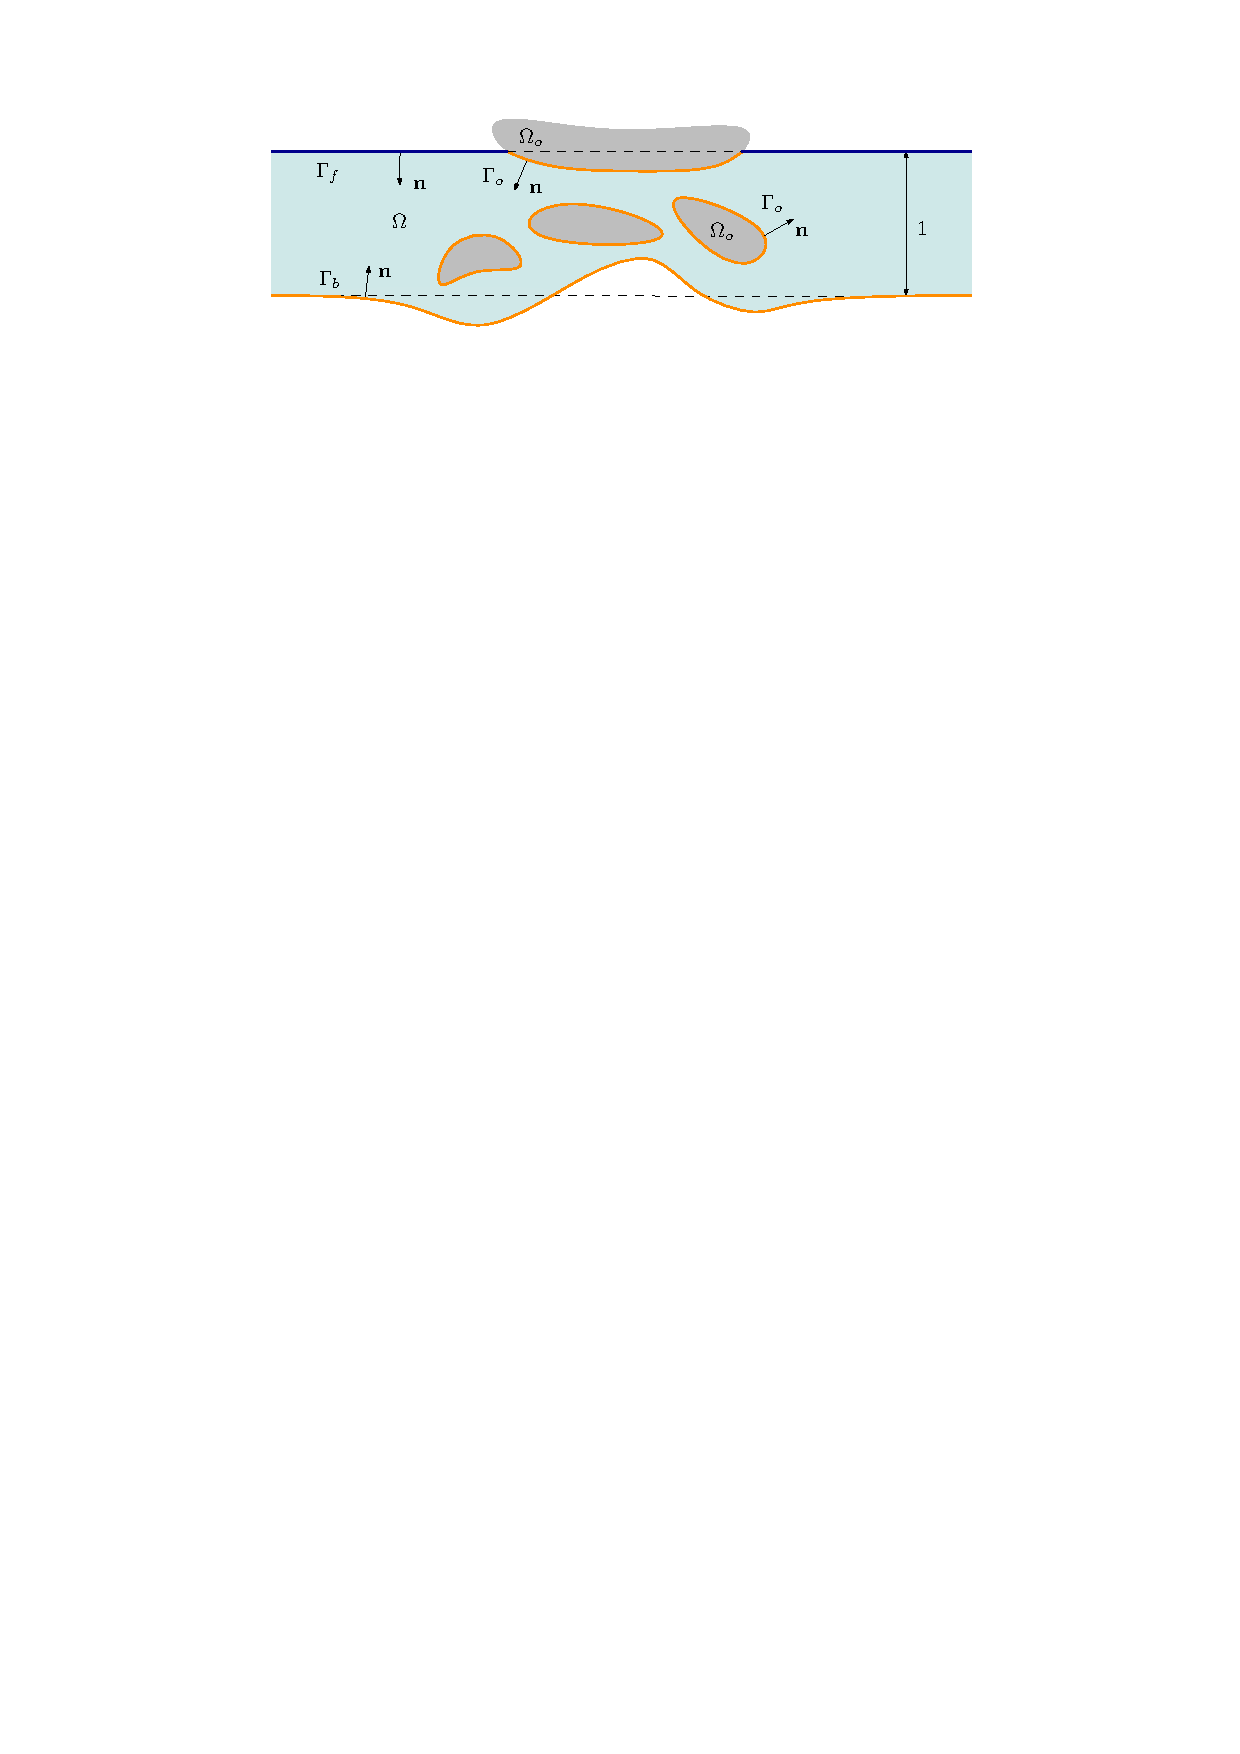
\includegraphics[scale=1]{WW_problem.pdf}
  \centering	  
  \caption{Schematics of the domain and main variables involved in the setup of water wave problem~\eqref{eq:water-waves-system} under consideration. \label{fig:schematic-geometry}}
\end{figure}

% Traditionally, in order to solve~\cref{eq:water-waves-system} by boundary
% integral equation methods, one must find an expression for its Green's function.
% Given the non-trivial nature of the boundary conditions, especially the radiating
% boundary condition at infinity given by ~\cref{eq:radiation-condition}, simple
% expressions for the Green's function are not available and intricate numerical
% procedures must be developed in order to efficiently compute the Green's
% function (see e.g.~\cite{xie2018comparison} for a recent review of
% three-dimensional methods, or ~\cite{mackay2021green} for the equivalent
% two-dimensional formulation). In this paper we propose a fundamentally different
% approach, where the water-waves system is first modified by the introduction of
% a perfectly matched layer absorbing propagative waves, and then the modified PDE
% is reformulated using boundary integral equations with the free-space Greens
% function of the transformed problem. 

% The main result of this paper is the following boundary integral equation for
% the analytic extension $\tvarphi$ of velocity potential $\varphi$:
% \begin{align*}
%   \frac{\tvarphi}{2} - \int_\Gamma \frac{\partial G_{\Delta}}{\partial \bn_\by}(\btau(\bx),\btau(\by)) \tvarphi(\by) \det(J(\by))\de s(\by) + \frac{\omega^2}{g}\int_{\Gamma_f} G_{\Delta}(\btau(\bx),\btau(\by)) \tvarphi(\by) \det(J(\by))\de s(\by) \\
%   = \int_{\Gamma} G_{\Delta}(\btau(\bx),\btau(\by)) \det(J(\by)) f(\by) \de s(\by), 
% \end{align*}
% where $\btau(\bx) = (\tau(\bx),x_2)$, is a certain \emph{complex-stretching},
% $J$ its Jacobian, and $G_{\Delta}$ is the free-space Green's function for the
% Laplace equation. The principal advantage of the proposed technique is that the
% fundamental solution of the PML-transformed problem requires only simple
% function evaluations (such as complex logarithms and square roots); the main
% drawback is that the (unbounded) free-surface must be discretized and truncated,
% therefore introducing additional degrees of freedom and a truncation error that
% must be controlled. 

In order to construct a suitable complex scaling for the problem~\eqref{eq:water-waves-system}, we rely on the analytic extension~$\varphi$. To justify the extension and gain insight into the construction of the complex stretching,  in what follows in this section we recall some classical results about the modal decomposition of $\varphi$ within semi-infinite strips of constant unit depth~\cite{kuznetsov2002linear,linton2001handbook}. Indeed, letting $L = \max(L_1,L_2)$, the exact solution $\varphi$ of~\eqref{eq:water-waves-system} admits a modal decomposition within the domain $\{|x_1|>L\}\times(-1,0)$. To define the modal decomposition we first introduce the sequence $\left\{\gamma_n\right\}_{n\geq 1}$, such that
%%%%%%%%%%%%%%%%%%%%%%%%%%%%%%%%%%%%%
\begin{equation}
  \label{eq:disp-evanescent}
  \gamma_n\tan(\gamma_n)=-\nu,\quad n\pi-\frac{\pi}{2}<\gamma_n <n\pi.
\end{equation}
%%%%%%%%%%%%%%%%%%%%%%%%%%%%%%%%%%%%%
Then one can prove that, with a suitable choice of the normalization constants
$(a_n)$, the functions $\{ u_n \}_{n\geq 0}$ defined by 
\begin{align}
\label{eq:transversemodes}
u_0(x_2)&=a_0\cosh(kx_2+k),&\\
u_n(x_2)&=a_n\cos(\gamma_nx_2+\gamma_n), \quad n\geq 1,
\end{align}
with $k>0$ being the solution of~\cref{eq:dispersion-relation} and $\gamma_n$ the solution of~\cref{eq:disp-evanescent}, form an orthonormal basis of $L^2([-1,0])$. Invoking the radiation condition~\cref{eq:radiation-condition} to select the correct behavior at $\pm \infty$, the following modal expansion for the solution $\varphi$ of~\eqref{eq:water-waves-system} can be readily obtained:
%
\begin{align}
  \label{eq:modaldecomp}
  \varphi(\bx) = \begin{cases}
  \displaystyle A_0^+u_0(x_2)\e^{ik(x_1-L)} + \sum_{n\geq 1}A_n^+u_n(x_2)\e^{-\gamma_n(x_1-L)} &\mbox{for }\bx\in (L,\infty)\times [-1,0],\medskip\\
  \displaystyle A_0^-u_0(x_2)\e^{-ik(x_1+L)} +\sum_{n\geq 1}A_n^-u_n(x_2)\e^{\gamma_n(x_1+L)} &\mbox{for }\bx\in (-\infty,-L)\times [-1,0],
  \end{cases}
\end{align}
where 
\begin{align}\label{eq:modal-decomp-amplitude}
  A_n^\pm=\int_{-1}^0\varphi(\pm L,x_2)\overline{u_n(x_2)}\de x_2,\quad n\geq 0.  
\end{align}

Let us mention that the well-posedness of~\eqref{eq:water-waves-system} can be studied by reducing the problem to a bounded domain via a DtN map approach derived from the modal expansion~\eqref{eq:modaldecomp}. Indeed, it can be established that the problem~\eqref{eq:water-waves-system} is well posed for all frequencies except for a countable set; see e.g.~\cite{thomas1977eigenfunction}.

Clearly, on each connected component of the exterior domain $\{|x_1|>L\}\times[-1,0]$ the velocity potential~$\varphi$ is a superposition of the outgoing surface wave and of infinitely many evanescent modes. 

\section{Complex-scaled boundary integral equation}\label{sec:complex-scaled-formulation}

In this section, we derive a complex scaled integral equation for solving~\cref{eq:water-waves-system} with the desirable 
property that its solutions are exponentially decreasing as $|x_1| \to \infty$.
Using the modal decomposition~\cref{eq:modaldecomp}, we show
in~\Cref{sec:complex-stretching} that the velocity potential $\varphi$ admits an analytic extension into the complex plane for $|x_1| > L$ (i.e. outside the support of the perturbations). Using the analytic extension of the modal decomposition, we then derive in~\Cref{sec:complex-scaled-bie} a modified water waves problem, as well as its boundary integral representation.

% and introduce a complex-valued function $\tau : \R \to \C$ so that $\tvarphi(\bx) = \varphi(\tau(x_1),x_2)$ is exponentially decaying as $|x_1| \to \infty$.
% We then derive in~\cref{sec:complex-scaled-bie} a complex-scaled integral representation formula, as well as an integral equation, for $\tvarphi$. 

\subsection{Complex stretching}\label{sec:complex-stretching}

The modal decomposition~\cref{eq:modaldecomp} can be used to study analytic
properties of $\varphi$ with respect to the coordinate $x_1$. More precisely,
for $x_1>L$ (resp. $x_1<-L$) the solution $\varphi$
of~\cref{eq:water-waves-system} has an analytic extension to complex values of its first variable
with a real part larger than $L$ (resp. smaller than $-L$). To see why this is so, let us consider for instance the side $x_1>L$. It is
clear that for any $N\in\N$, the finite sum
\begin{align}
  A_0^+u_0(x_2)\e^{ik(z_1-L)}+\sum_{n= 1}^NA_n^+u_n(x_2)\e^{-\gamma_n(z_1-L)}
\end{align}
is well-defined for complex values of $z_1$, and is a holomorphic function of
$z_1$. Moreover, it converges when $N\to +\infty$,
uniformly in all compact subsets of $\real(z_1)>L$, to a function that we denote (with a slight abuse of notation) by $\varphi(z_1,x_2)$.  Finally, thanks to Morera's theorem, a uniform limit of a sequence of holomorphic functions is itself holomorphic, so we conclude that  $z_1\mapsto\varphi(z_1,x_2)$ is analytic within $\real(z_1)>L$. The exact same argument applies to the analytic extension $z_1\mapsto\varphi(z_1,x_2)$ for $\real(z_1)<-L$.

% We are interested in the analytic extension of $\varphi$ when it
% is exponentially decaying at infinity, for such a behavior facilitates the truncation of the curves $\Gamma_b$ and $\Gamma_f$. This means we consider only the analytic extension of $\varphi$ on $\left\{\widetilde{x}_1 \in C \right\}$ for $\Re(x_1)>L$  (resp. $\Re(x_1)<-L$) only for $\imag(x_1)>0$ (resp. $\imag(x_1)<0$) so that the propagating mode, given by the first term in~\cref{eq:modaldecomp}, becomes exponentially decaying at infinity.

It follows then  by the analyticity of $\varphi$ that
\begin{align}  
  \label{eq:pml-laplace-equation}
  \left( \partial_{z_1}^2 + \partial_{x_2}^2 \right) \varphi(z_1,x_2) &=0, \quad (z_1,x_2) \in \{|\real z_1 | > L \} \times [-1,0].
\end{align}
We now introduce a (continuous) stretching path $\tau : \R \to \C$ along which the transformed function 
\begin{equation}\label{eq:transf_eq}
\tvarphi(x_1,x_2) := \varphi(\tau(x_1),x_2)    
\end{equation} decays exponentially fast as $|x_1| \to \infty$. In view of the modal decomposition~\cref{eq:modaldecomp}, the following conditions guarantee the exponential decay of $\tvarphi(\cdot,x_2)$:
\begin{subequations}
\label{eq:tau-conditions}
\begin{align}
    \imag\left(\tau(x_1)\right) &> 0 \quad \mbox{for} \quad x_1 > L\\
    \imag\left(\tau(x_1)\right) &< 0 \quad \mbox{for} \quad x_1 < -L
\end{align}        
\end{subequations}
Furthermore, in order to recover the original solution to~\cref{eq:water-waves-system} for $|x_1| < L$, we require
\begin{subequations}
    \begin{align}
        \tau(x_1) = x_1 \quad \mbox{for} \quad |x_1|<L. \tag{\ref{eq:tau-conditions}c}
        \label{eq:tau-condition-identity}
    \end{align}
\end{subequations}
Finally, we suppose that
\begin{subequations}
\begin{align}
    0 < c < \real(\tau'(x_1)) < C < \infty \quad \mbox{for} \quad x_1 \in \R \tag{\ref{eq:tau-conditions}d}
    \label{eq:tau-condition-real}
\end{align}
\end{subequations}
which implies that $\tau$ is injective. 

A simple application of the chain rule then yields $\partial_{z_1} \varphi(\tau(x_1),x_2) = \partial_{x_1} \tvarphi(x_1,x_2)/\tau'(x_1) $ 
% and $\partial^2_{z_1} \varphi(\tau(x_1),x_2) = \partial_{x_1}[\partial_{x_1} \tvarphi(x_1,x_2)/\tau'(x_1)]/\tau'(x_1) $
and, therefore, in view of~\eqref{eq:pml-laplace-equation},  $\tvarphi$ defined in~\eqref{eq:transf_eq} satisfies
\begin{subequations}
\begin{align}
  \label{eq:pml-laplace-real}
  \nabla \cdot (A(\bx) \nabla \tvarphi) &= 0  \quad \mbox{with} \quad A(\bx) :=   
  \begin{bmatrix}
    \tau'(x_1)^{-1} & 0 \\
    0 & \tau'(x_1)
  \end{bmatrix}, \quad \bx \in \Omega.
\end{align}
\label{eq:water-waves-system-pml}
\end{subequations}
(We have chosen a matrix formalism to simplify the discussion in the subsequent section.) Note that by~\cref{eq:tau-condition-identity}, $\tau' = 1$ for $|x_1| < L$,  so~\cref{eq:pml-laplace-real} becomes the Laplace equation in that case. Finally, we note that because $f_1$ and $f_2$, as well as the geometrical perturbations, vanish for $|x_1|>L$, it can be easily shown that $\tvarphi$ satisfies the same boundary conditions:
%
\begin{subequations}
\begin{align}
    \label{eq:pml-free-surface-bc}
    \nabla \tvarphi(\bx) \cdot \bn(\bx) + \nu\tvarphi(\bx)&=f_1(\bx), \quad \bx \in \Gamma_f:=\Gamma_s\setminus\overline\Omega_o, \tag{\ref{eq:water-waves-system-pml}b}\\
    \label{eq:pml-solid-bc}  
    \nabla \tvarphi(\bx) \cdot \bn(\bx) &=f_2(\bx), \quad \bx \in \Gamma_b \cup \Gamma_o. \tag{\ref{eq:water-waves-system-pml}c}
    % \\
    % \label{eq:radiation-condition-pml}  
    % \lim_{x_1 \to \pm \infty} \partial_{x_1} \tvarphi(\bx) \mp i k \tau'(x_1) \tvarphi(\bx)  &= 0.
    % \tag{\ref{eq:water-waves-system-pml}d}
\end{align}
\end{subequations}
It is worth mentioning that the radiation condition~\cref{eq:radiation-condition} is replaced by the fact that $\tvarphi$ is exponentially decaying. Equations \cref{eq:water-waves-system-pml} comprise the PML-transformed water waves system that we seek to solve in lieu of the original system~\cref{eq:water-waves-system}.

\subsection{Boundary integral equation}\label{sec:complex-scaled-bie}
In order to recast the problem as a BIE by leveraging fundamental potential theory results, we first show that our PDE~\cref{eq:pml-laplace-real} is strongly elliptic in the sense of \cite{mclean2000strongly}. Indeed, given the form of the matrix function $A$ introduced in~\cref{eq:pml-laplace-real} and the stretching path property~\cref{eq:tau-condition-real}, it follows that
\begin{align}
    \real(\xi^* A \xi) = \real\left( \frac{1}{\tau'} |\xi_1|^2 + \tau' |\xi_2|^2 \right) > \min\left(c,\frac{c}{C}\right) |\xi|^2,\quad \xi \in \C^2,
\end{align}
which shows the desired property. 

% Given the form of the matrix function $A$ introduced in~\cref{eq:pml-laplace-real} and the stretching path property~\cref{eq:tau-condition-real}, it follows that
% \begin{align}
%     \real(\xi^* A \xi) = \real\left( \frac{1}{\tau'} |\xi_1|^2 + \tau' |\xi_2|^2 \right) > \min\left(c,\frac{c}{C}\right) |\xi|^2.
% \end{align}
% This means that the PDE~\cref{eq:pml-laplace-real} is strongly elliptic and, as such, the general theory of boundary integral equation can be applied~\cite{mclean2000strongly}. 

A crucial aspect of the subsequent BIE formulation is the following explicit relationship between the free-space Green's function $\widetilde{G}$ associated with~\cref{eq:pml-laplace-real}, and Laplace's fundamental solution $G$, along with the transformation $\tau$ (see~\Cref{sec:fundamental-solution}):
\begin{align}
  \label{eq:complex-Green-function}
\widetilde{G}(\bx,\by) := G(\btau(\bx),\btau(\by)) = -\frac{1}{4\pi}\log \left( (\tau(x_1) - \tau(y_1))^2 + (x_2 - y_2)^2 \right),
\end{align}
where the principal logarithm is used, with a branch cut on the negative real line, and where, for the sake of compactness of notation, we have introduced the vector-valued transformation 
$$\btau(\bx) := (\tau(x_1),x_2) : \R^2 \to \C \times \R.$$ %be the vector-valued transformation introduced for notation compactness. 

With these definitions at hand, we are in a position to derive the boundary integral representation for $\tvarphi$, defined in~\eqref{eq:transf_eq}, over the (unbounded) domain $\Omega$. We then begin by considering the truncated domain $\Omega_M := \left\{\bx \in \Omega : |x_1| <  M \right\}$, $M>0$. On $\Omega_M$, the following integral representation formula holds~\cite{mclean2000strongly}:
\begin{align}
  \label{eq:greens-representation-bounded}
  \tvarphi(\br) = \mathcal{D}_{\partial \Omega_M}[\tvarphi](\br) - \mathcal{S}_{\partial \Omega_M}[\nabla \tvarphi \cdot A \bn](\br), \quad \br \in \Omega_M,
\end{align}
where $\mathcal{S}_\Sigma$ and $\mathcal{D}_\Sigma$ denote respectively the single- and double-layer potentials  as
\begin{subequations}
\begin{align}
    \label{eq:SL-pot}
    \mathcal{S}_{\Sigma}[\sigma](\br) &:= \int_\Sigma \widetilde{G}(\bx,\by) \sigma(\by) \de s(\by)\quad\text{and}\\
    \label{eq:DL-pot}
    \mathcal{D}_{\Sigma}[\sigma](\br) &:= \int_\Sigma \left( \nabla_{\by} \widetilde{G}(\bx,\by) \cdot A(\by)\bn(\by) \right) \sigma(\by) \de s(\by),\quad\bx\in\R^2\setminus\Sigma,
\end{align}
\label{eq:potentials}
\end{subequations}
where $\Sigma$ stands for a generic sufficiently regular (Lipschitz) curve. 

% In what follows we consider $\tau(x_1,x_2) = \mu_r(x_1) + i \mu_i(x_1,x_2)$,
% where $\mu_r : \R \to \R$ represents a \emph{real-stretching} and $\mu_i : \R^2 \to \R$
% is the \emph{complex-stretching}. Furthermore, we will always assume that
% $\tau(x_1,x_2) = x_1$ for $|x_1|<L$, so that $\tvarphi(\bx) = \varphi(\bx)$ for
% $|x_1|<L$. 
% Some comments are in order regarding the somewhat unusual choice of
% complex-stretching $\tau$. First the real stretching $\mu_r$, usually taking to
% be the identity $\mu_r(x_1) = x_1$, will be used to damp the evanescent modes
% should their decay rate become too slow compared to the complexified propagative
% wave. The dependency $\mu_i$ on the transversal variable $x_2$, on the other
% hand, is related to the fact that we since the waves are localized at the
% surface, we can consider \emph{non-orthogonal} PMLs so that $\varphi = \tvarphi$
% on a larger domain; that is, by relaxing the complex stretching with the depth
% variable $x_2$, we may recover the correct solution on domain larger than if
% $\partial_{x_2} \mu_i = 0$. 
Using the fact that $\tvarphi$ decays exponentially fast as $|x_1| \to \infty$, while the integral kernels in~\cref{eq:greens-representation} grow at most logarithmically, the contribution from the lateral curves $\{ \pm M\} \times
[-1,0]\subset\partial\Omega_M$ in~\eqref{eq:greens-representation-bounded} decays exponentially fast as $M \to \infty$. As such, we may
replace $\Omega_M$ by its limit $\Omega$ in~\cref{eq:greens-representation-bounded}, yielding the following integral representation:
\begin{align}
  \label{eq:greens-representation}
  \tvarphi(\br) = \mathcal{D}_{\Gamma}[\tvarphi](\br) - \mathcal{S}_{\Gamma}[\nabla \tvarphi \cdot A \bn](\br), \quad  \br \in \Omega,
\end{align}
where $\Gamma := \partial \Omega = \Gamma_b \cup \Gamma_o \cup \Gamma_f$. 

It is worth mentioning that an integral representation on the unbounded curve~$\Gamma$, such as~\cref{eq:greens-representation}, can only be obtained for $\tvarphi$, and not for $\varphi$. In fact, in the absence of a complex-stretching, equation~\cref{eq:greens-representation} ceases to make sense because $\varphi$ does not decay, and the single-layer kernel exhibits a logarithmic growth, meaning that the integrals are not convergent (even in the conditional sense). This is a fundamental difference from the Helmholtz equation, where the decay of the Green's function and of the scattered field suffices to render integrals over unbounded interfaces conditionally convergent (but not absolutely so). 

Next, to obtain an integral equation for $\tvarphi$ over $\Gamma$, we evaluate the limit $\Omega \ni \br \to \bx \in \Gamma$ in~\cref{eq:greens-representation}. Taking into account the jump condition of the
the double-layer potential~\eqref{eq:DL-pot} across $\Gamma$~\cite{mclean2000strongly}, we arrive at %the well-known Green's identity:
\begin{align}
  \label{eq:greens-formula}
  \frac{\tvarphi(\bx)}{2} &=  D_{\Gamma}[\tvarphi](\bx) - S_{\Gamma}[\nabla \tvarphi \cdot A \bn](\bx), \quad \bx \in \Gamma,
\end{align}
where $S_{\Gamma}$ and $D_{\Gamma}$ are respectively the single- and double-layer operators,
defined as
\begin{subequations}
  \label{eq:calderon-operators}
  \begin{align}
  \label{eq:SL-operator}  
  S_{\Gamma}[\sigma](\bx) &:= \int_\Gamma \widetilde{G}(\bx,\by) \sigma(\by) \de s(\by) \quad\text{and}\\
  \label{eq:DL-operator}  
  D_{\Gamma}[\sigma](\bx) &:= {\rm p.v.}\! \int_\Gamma\left(\nabla_{\by} \widetilde{G}(\bx,\by) \cdot A(\by)\bn(\by) \right)
  \sigma(\by) \de s(\by), \quad \bx \in \Gamma.
\end{align}\label{eq:BIOS}\end{subequations}
The letters p.v. in front of the integral sign in~\cref{eq:DL-operator} refer to the fact that the integral must be interpreted in the sense of the Cauchy principal value.

Note that the double-layer kernel is given in explicit terms by
\begin{align}
  \label{eq:complex-double-layer-kernel}
\nabla_{\by}\widetilde{G}(\bx,\by) \cdot A(\by)\bn(\by) = \tau'(y_1)\frac{\partial G}{\partial\bn_{\by}}(\btau(\bx),\btau(\by)) = \frac{\tau'(y_1)(\btau(\bx)-\btau(\by)) \cdot \bn(\by)}{2\pi (\btau(\bx) - \btau(\by)) \cdot (\btau(\bx) - \btau(\by))},
\end{align}
which is simply a (complex) multiple of Laplace's free-space double-layer kernels evaluated at the complex points $\btau(\bx)$ and $\btau(\by)$. Furthermore, under the additional assumption that~$\Gamma$ and $\btau$ are smooth at $\bx$, we can expand
\begin{align}
\btau(\by) &= \btau(\bx) + J(\bx) (\bx - \by) + \mathcal{O}(|\bx - \by|^2), \\
\bn(\by) &= \bn(\bx) + \mathcal{O}(|\bx - \by|)
\end{align}
where 
\begin{align}
    J(\bx) = \begin{bmatrix}
        \tau'(x_1) & 0\\
        0     & 1
    \end{bmatrix}
\end{align}
is the Jacobian matrix. Using then the fact that $J(\bx) \bn(\bx) = \bn(\bx)$ for any $\bx \in \Gamma$ since $J$ is either the identity (outside the PML) or $\bn$ points in the $x_2$ direction (inside the PML), we have that
\begin{align}
\nabla_{\by}\widetilde{G}(\bx,\by) \cdot A(\by)\bn(\by) = \frac{\tau'(x_1) (\bx - \by) \cdot \bn(\bx)}{J(\bx)(\bx - \by)\cdot J(\bx)(\bx - \by)} + \mathcal{O}(1) \quad \mbox{as} \quad \by \to \bx,
\end{align}
Since $(\bx - \by) \cdot \bn(\bx) = \mathcal{O}(|\bx - \by|^2)$ as $\Gamma \ni \by \to \bx \in \Gamma$ for a smooth curve, this means in particular that double-layer kernel~\cref{eq:complex-double-layer-kernel} is a bounded function at $\by = \bx$, and therefore the principal value in~\cref{eq:DL-operator} is not necessary in such cases. 

With the validity of the representation formula~\cref{eq:greens-representation}
established, and the availability of the free-space fundamental solution~\cref{eq:complex-Green-function}, we can
now formally derive a BIE for $\tvarphi$. Indeed, using the boundary conditions~\cref{eq:pml-free-surface-bc,eq:pml-solid-bc} to replace
$\nabla \tvarphi \cdot A \bn = \tau' \tvarphi \cdot \bn$ in favor of $\tvarphi$ in~\cref{eq:greens-formula}, we arrive at 
%
\begin{align}
  \label{eq:BIE-long}
  -\frac{\tvarphi(\bx)}{2} + D_{\Gamma}[\tvarphi](\bx) + \nu S_{\Gamma_f}\left[\tau'\tvarphi\right](\bx) &= S_{\Gamma_f}[f_1](\bx) + S_{\Gamma_b \cup \Gamma_o}[f_2](\bx), \quad \bx \in \Gamma.
\end{align}
%

To further simplify the notation, we introduce a ``global" impedance-like coefficient $\alpha : \Gamma \to \R$, as well as a ``global" source $f : \Gamma \to \R$ given by:
\begin{align}
    \alpha(\bx) = \nu\mathbbm{1}_{\Gamma_f}, \quad f(\bx) = f_1(\bx) \mathbbm{1}_{\Gamma_f} + f_2(\bx) \mathbbm{1}_{\Gamma_o \cup \Gamma_b},
\end{align}
where $\mathbbm{1}_{\Sigma}$ denotes the indicator function over a domain $\Sigma$. Equation~\cref{eq:BIE-long} is then rewritten in a more compact form as 
%
\begin{align}
  \label{eq:BIE}
  -\frac{\tvarphi(\bx)}{2} + D_{\Gamma}[\tvarphi](\bx) + S_\Gamma\left[\alpha\tau'\tvarphi\right](\bx) &= S_{\Gamma}[f](\bx), \quad \bx \in \Gamma.
\end{align}

\begin{remark}[Indirect formulation]
  An alternative method to derive a boundary integral equation
  for~\cref{eq:water-waves-system} is to use an \emph{indirect} approach, where
  we seek the velocity potential in the form $\widetilde{\phi}(\br) =
  \mathcal{S}[\sigma](\br)$, with $\sigma$ being an unknown density. This leads
  to an equation similar to~\cref{eq:BIE}. We have chosen to pursue a
  \emph{direct} formulation since then it follows directly that the unknown
  $\tvarphi$ is exponentially decreasing as $|x_1| \to \infty$. 
\end{remark}

\begin{remark}[Resonance frequencies]\label{rem:linear_eig_problem}
Interestingly, the proposed complex-scaled formulation depends linearly on  $\nu$. This contrasts formulations based on the water-waves Green's function, for which the dependency on $\nu$ appears (non-linearly) inside the kernels of the integral operators. This means, in particular, that we may solve a generalized linear eigenvalue problem to find either complex or real resonances (should they exist). We will explore this advantage of our method to compute complex resonances in~\cref{sec:numerical-results}. 
\end{remark}


In the subsequent sections, we will present the development of a Nystr\"om method for the numerical approximation of solutions to~\eqref{eq:BIE}. 
% Before delving into the method, we acknowledge some important theoretical aspects that arise from the proposed approach which could not be addressed by the authors in the present contribution.

% Consider now $u(\br) = \mathcal{S}[g](\br)$ with $u = 0$ on $\overline{\Omega}$. Then $g$ is the jump in the Neumann trace of $u$, i.e. $u = \gamma_1^+ u - \gamma_1^- u$. To show that $u = 0$ on $\R^2 \setminus \Omega$, we proceed as follows. First, ...
% \textbf{TODO: I am blocked. I want to assume that $\sigma$ decays exponentially in what follows, but I do not know how to justify that...}

% Then, since $u$ is a solution of~\cref{eq:pml-laplace-real}, it follows that 
% \begin{align}
%     \int_{\Omega_M} \nabla\cdot \left(A \nabla u\right) u^* \de \by = \int_{\partial\Omega_M} \left( \nabla u \cdot A \bn \right) u^* \de s- \int_{\Omega_M} (\nabla u)^* A \nabla u \de \by = 0
% \end{align}

% The behavior of $u$ at infinitely can be readily obtained from the representation 
% \begin{align}
%     \lim_{|\br| \to \infty} u(\br) = G(\btau(\bx)
% \end{align}

% Interestingly, the proposed complex-scaled formulation depends linearly on the frequency $\omega$. This contrasts formulations based on the water-waves Green's function, for which the $\omega$ dependency appears (non-linearly) inside the kernels of the integral operators. This means, in particular, that we may solve a generalized linear eigenvalue problem to find either complex or real resonances (should they exist). We will explore this advantage of our method to compute resonant frequencies in~\cref{sec:numerical-results}. 

% % Note that although we required $\tau$ to be defined in all of $\Omega$ when deriving our modified water-waves problem, only its trace on $\Gamma$ is used in
% % the integral equation~\cref{eq:BIE}. This means there are infinitely many
% % volumetric PMLs yielding the same integral equation (but with different integral
% % representations). Because we are mostly interested in what happens at the
% % free surface, we focus primarily on the value of $\tau$ there, i.e. $\tau(x_1,0)$. 

% In the following section, we discuss some details related to the truncation and numerical discretization of the (singular) integral operators in~\cref{eq:BIE}.

% % \begin{remark}[Irregular frequencies]
% %   It remains unclear whether~\cref{eq:BIE} is uniquely solvable for all
% %   frequencies $\omega$ corresponding to a well-posed problem (i.e. $\omega$ such
% %   that ~\cref{eq:water-waves-system} has a unique solution).
% %   In other words, we do not know if~\cref{eq:BIE} suffers from
% %   \emph{irregular frequencies}. The usual argument for constructing irregular frequencies $\lambda$ (see e.g.~\cite[section 8.8.1]{mei2005theory}), based on an interior eigenvalues problem of the type
% %   \begin{subequations}
% %   \begin{align}
% %     \Delta \Psi &= 0, \quad \br \in \Omega',\\
% %     \Psi &= 0, \quad \bx \in \Gamma_o,\\    \nabla \Psi + \lambda \Psi &= 0, \quad \bx \in \partial \Omega' \setminus \Gamma_o, 
% %   \end{align}
% %   \end{subequations}
% %   where $\Omega'$ is the domain bounded by the piercing object and the free surface, and $\Gamma_o$ is the obstacle's boundary, appears to fail due to the presence of an unbounded surface in~\cref{eq:BIE}. 
% % \end{remark}

% \begin{remark}[Indirect formulation]  
%   An alternative method to derive a boundary integral equation
%   for~\cref{eq:water-waves-system} is to use an \emph{indirect} approach, where
%   we seek the velocity potential in the form $\widetilde{\phi}(\br) =
%   \mathcal{S}[\sigma](\br)$, with $\sigma$ being an unknown density. This leads
%   to an equation similar to~\cref{eq:BIE}. We have chosen to pursue a
%   \emph{direct} formulation since then it follows directly that the unknown
%   $\tvarphi$ is exponentially decreasing as $|x_1| \to \infty$. 
% \end{remark}

% \begin{table}
%   \centering
%   \begin{tabular}{l l l}
% \toprule
%     \textbf{Notation/Definition} & \textbf{Meaning} & \textbf{Domain$\rightarrow$Range} \\
%     \hline
%     $\bx=(x_1,x_2)$  & Spatial variable & $\R^2$ \\
%      $\tau(\bx)=\mu_r(x_1) + \mu_i(\bx)$ & PML change of variables & $\R^2 \to \C$\\
%      $\btau(\bx)=(\tau(\bx),x_2)$ & Vector valued PML& $\R^2 \to \C \times \R$\\
%     $G(\bx,\by)$  & Laplace free-space Green function & $\R^2 \times \R^2 \to \C$ \\
%     $\widetilde{G}(\bx,\by) = G(\btau(\bx),\btau(\by))$  & PML-transformed Green function & $\R^2 \times \R^2 \to \C$ \\
%     $\tau_{i,j} =\pder{\tau_i}{x_j}$  & Partial derivative & $\R  \to \C$\\
%     % $J = \pder{\tau}{\bx}$  & Jacobian matrix & $\C^{2\times 2}$\\
%   \end{tabular}
%   \caption{Notation and symbols commonly used in the paper.}
%   \label{tab:notation}
% \end{table}

% \begin{remark}[Double-layer singularity]
%   For smooth surfaces, the double-layer operator~\cref{eq:DL-operator} is weakly
%   singular because $(\tau(\bx) - \btau(\by)) \cdot \bn_{\by} = \mathcal{O}(|\bx
%   - \by|^2)$ as $\Gamma \ni \by \to \bx \in \Gamma$.
% \end{remark}

\section{Numerical method}\label{sec:Nyst_meth}

In this section, we provide the details of the discretization scheme employed, as
well as the concrete choice of the (linear) PML function used and the parameters involved. %While a rigorous analysis of the truncation error remains missing, 
We also present an argument for the consistency of the truncated BIE which includes an integral equation for the error, that exhibits a right-hand-side that vanishes exponentially as $M\to\infty$. The numerical examples of~\Cref{sec:numerical-results} demonstrate that, as expected, the truncation errors decay exponentially with respect to the length of the PML layer.

In order to discretize~\cref{eq:BIE}, we proceed in two steps. First, after a choice of PML function $\tau$ in~\eqref{eq:tau-conditions} has been made, the infinite boundary $\Gamma$ is truncated to a finite curve $\Gamma_M = \{ \bx \in \Gamma : |x_1| < M \}$. Second, the resulting integral equation over $\Gamma_M$ is discretized using a Nyström scheme, wherein a composite $P$-point Gauss-Legendre quadrature rule is used to approximate the integrals over
$\Gamma_{M}$. A correction, which  accounts
for the singular and nearly-singular interactions arising in the numerical discretization of the underlying integral operators, is obtained by means of a
Gauss-Kronrod adaptive quadrature; more details are given in~\Cref{sec:discretization-error}. 

The particular choice of the BIE discretization here developed overcomes certain limitations of existing more established Nystr\"om methods. For instance, the spectrally accurate Martensen-Kussmaul approach~\cite[section 3.6]{colton1998inverse} becomes numerically unstable in the current setting due to the underlying kernel splitting  involving complex arguments~\cite{lu2014efficient}. Other approaches, such as the Density Interpolation Method~\cite{perez2019harmonic,faria2021general}, developed by some of the authors and collaborators, does not handle open curves such as the ones that arise in the current BIE formulation. The hybrid Gauss-trapezoidal quadrature rule of Alpert~\cite{alpert1999hybrid}, on the other hand, can in principle be used in the current setting and was the choice of spatial discretization used by Lu et al. in~\cite{lu2018perfectly}.

Throughout this section, we will use $\tvarphi_{M,h}$ to denote the approximate solution over $\Gamma_{M}$ using a $P$-point quadrature rule on elements of approximate size $h$, where the dependency on $P$ is omitted for notational simplicity. 

\subsection{Domain truncation}\label{sec:truncation}

%To understand the truncation errors, 
To ensure a clear and concise presentation, we will focus exclusively on linear PMLs. Consequently,~$\tau$ is given by
%For the sake of presentation simplicity, we here focus on linear PMLs, whereby $\tau$ is given by
%%%%%%%%%%%%%%%%%%%%%%%%%
\begin{align}
    \label{eq:linear-pml}
  \tau(x_1) &= x_1 + i 
  \begin{cases}
    c (x_1+a), & x_1 \leq -a, \\
    0, & |x_1| < a, \\
    c (x_1 - a) & x_1 \geq a,
\end{cases}
\end{align}
%%%%%%%%%%%%%%%%%%%%%%%%%
where $a>0$ is a parameter controlling the start of the complex stretching, while the parameter $c>0$ controls its slope. We know from~\cref{eq:modaldecomp} that $\tvarphi(x_1,x_2) = \varphi(\tau(\bx),x_2)$ admits the following
modal decomposition for $x_1 > L$:
\begin{align}
  \label{eq:modal-decomp-extension}
  \tvarphi(x_1,x_2) =  \displaystyle A_0^+u_0(x_2)\e^{-ck(x_1-a)} \e^{ik(x_1-L)} + \sum_{n\geq 1}A_n^+u_n(x_2)\e^{-\gamma_n(x_1-L)}\e^{-ic\gamma_n(x_1-a)}
\end{align}
with the coefficients $A_n^+$ given in~\cref{eq:modal-decomp-amplitude}. This shows that 
\begin{align}
    \tvarphi(x_1,x_2) \sim \mathcal{O}(\e^{-\min(ck,\gamma_1) x_1}) \quad \mbox{as} \quad x_1 \to \infty.
    \label{eq:decay-rate}
\end{align}
A similar argument holds for $x_1 \to -\infty$, and thus $\tvarphi$ decays exponentially as $|x_1| \to \infty$. 

% Our somewhat unusual choice of a two-layered piece-wise linear PML can be
% motivated as follows. The propagating mode behaves as $e^{ik|x_1|}$, and
% therefore a complex-stretching $\mu_i$ is needed to convert such waves into a
% decaying exponential. With~\cref{eq:pml-with-stretching}, it is easy to see that
% the propagating mode now behaves as $e^{-kc_i|x_1|}e^{ikx_1}$, and thus the complex
% stretching achieves the (main) goal of rendering $\tvarphi$ exponentially
% decaying. As it turns out, however, the exponential decay rate of $\tvarphi$ may
% be much slower than $\mathcal{O}(e^{-k c_i |x_1|})$ as $|x_1| \to \infty$ due to
% the presence of the evanescent modes. More precisely, should $\gamma_1$ be
% smaller than $k c_i$, truncation errors will be dominated by the evanescent
% modes and $\tvarphi \sim \mathcal{O}(-\gamma_1|x_1|)$ as $|x_1| \to \infty$.
% This motivates the inclusion of the real stretching factor $\mu_r$ whose main
% goal is to accelerate the decay of the evanescent modes. Since $n\pi - \pi/2 <
% \gamma_n d < n \pi + \pi/2$, $c_r = d$ is a natural scale for the transformation
% as it yields evanescent modes which decay at an $\mathcal{O}(1)$ rate regardless
% of the depth. It should be noted that the real stretching increases the
% frequency of the propagating mode, an undesirable consequence for it increases the truncation error when the solution is approximated numerically on a fixed grid. Because of that, the approach employed consists of
% first attenuating the oscillatory part (without increasing its frequency), and
% only then introducing the real stretching factor for handling the evanescent modes. We emphasize that the second real stretching layer is not strictly necessary for a (fixed) finite depth for the solution still decays exponentially in its absence, but it may be used to further reduce the truncation error at a modest computational cost. 

Given the exponential decay of $\tvarphi$, we replace the integral equation~\cref{eq:BIE} by its truncated version
\begin{align}
  \label{eq:BIE-truncated}
  -\frac{\tvarphi_{M}(\bx)}{2} + D_{\Gamma_{M}}[\tvarphi_M](\bx) + S_{\Gamma_{M}}\left[\alpha\tau'\tvarphi_M\right](\bx) &= S_{\Gamma_M}[f](\bx), \quad \bx \in \Gamma_M.
\end{align}
Note that this domain truncation is equivalent to fixing the value of $\tvarphi$
to be exactly zero for $|x_1| > M$. Subtracting~\cref{eq:BIE-truncated} from~\cref{eq:BIE}, it is straightforward to see that the truncation error $\mathcal{E}_M(\bx) := \tvarphi(\bx) - \tvarphi_M(\bx)$
satisfies the following second-kind integral equation:
\begin{align}
  \label{eq:BIE-truncated-error}
  -\frac{\mathcal{E}_M(\bx)}{2} + D_{\Gamma_{M}}[\mathcal{E}_M](\bx) + S_{\Gamma_{M}}\left[\alpha \tau' \mathcal{E}_M\right](\bx) &= -D_{\Gamma^c_{M}}[\tvarphi](\bx) - S_{\Gamma^c_{M}}\left[\alpha \tau' \tvarphi\right](\bx), \quad \bx \in \Gamma_M,
\end{align}
where $\Gamma_M^c = \Gamma \setminus \Gamma_M$. Because of the exponential decay of $\tvarphi$, it follows that the right-hand side is exponentially small in $M$ as $M \to \infty$, which shows the consistency of the truncation technique.  To conclude that $\mathcal{E}_M$ is also exponentially small, a stability result of the type
\begin{align}
    || \mathcal{L}^{-1}_M ||_{L^2(\Gamma_M) \to L^2(\Gamma_M)} \leq M^q, \quad    \mathcal{L}[\sigma] := - \frac{\sigma}{2} + D_{\Gamma_M}[\sigma] + S_{\Gamma_{M}}[\alpha \tau' \sigma]
\end{align}
is needed as $M \to \infty$, with $q > 0$ independent of $M$. Although such a result is lacking in our analysis, the numerical tests of~\Cref{sec:numerical-results} suggest that the truncation errors are exponentially small in $M$. 

\begin{remark}[PML parameters]
While it may be tempting to take $c$ large in~\cref{eq:linear-pml} so as to improve the exponential decay of $\tvarphi$, consideration of discretization errors ($\tvarphi$ has to be approximated on a grid) will typically put bounds on the size of $c$. Even if we assume, as is the case in this paper, that the same grid size is used inside and outside the PML layer, the question of determining the ``optimal'' PML parameters is subtle and depends closely on the discretization scheme employed, for one seeks to balance truncation and discretization errors. In this paper, we simply take $c=1$, and avoid questions related to an optimal choice of PML parameters. 
\end{remark}

% Finally, given a desired tolerance $\epsilon$ and the strength of the PML $c_i$
% (recall that $c_r = d$), a simple heuristic is to chose $\ell_i \sim
% -\log(\epsilon)/(k c_i)$, and $\ell_r \sim \log(\epsilon) ( \gamma_1/(k c_i) -
% 1) / \gamma_1d$.

\subsection{Singular and nearly-singular integration}
\label{sec:discretization-error}

With a truncated curve $\Gamma_M$ at hand, we are now ready to discretize the integral operators in~\cref{eq:BIE-truncated}. To this end, we assume that the boundary $\Gamma_M$ is covered by $N$ non-overlapping elements $\left\{ \mu_n \right\}_{n=1}^N$ of approximate size $h$; i.e. 
\begin{align}
  \Gamma_M = \bigcup_{n=1}^N \overline{\mu}_n.
\end{align}
For each element $\mu_n$, a $\mathcal{C}^\infty$ bijection $\chi_n : [0,1] \to \overline{\mu_n}$ is assumed known.

On each $\mu_n$, a $P$-point Gauss-Legendre quadrature rule $\mathcal{Q}_n = \left\{ \left( \bx_{p,m}, w_{p,m} \right) \right\}_{p=1}^P$ is constructed by mapping the quadrature on the reference segment $[0,1]$ to $\overline{\mu_m}$ using $\chi_m$. A composite quadrature $\mathcal{Q}$ for $\Gamma_{M}$ is then obtained by collecting the element quadratures:
\begin{align}
  \mathcal{Q} = \left\{ \mathcal{Q}_n \right\}_{n=1}^N = \left\{ \left\{ \left( \bx_{p,n}, w_{p,n} \right) \right\}_{p=1}^P \right\}_{n=1}^N.
\end{align}

Given an element index $p$ and a local quadrature index $n$, it will be sometimes convenient to use a linear index $i = n(P-1) + p$, $1 \leq i \leq NP$, to refer to the node $\bx_{p,n}$ as $\bx_i$. With this linear index, the boundary quadrature can be alternatively written as 
\begin{align}
  \mathcal{Q} = \left\{ \left( \bx_{i}, w_{i} \right) \right\}_{i=1}^{NP}.
\end{align}

Using a Nyström discretization, the integral operators in~\cref{eq:BIE} are approximated using the quadrature $\mathcal{Q}$, and equality is enforced (strongly) at the quadrature nodes. This yields the following discrete linear system for $\tvarphi_{i} \approx\tvarphi_M(\bx_i)$:
\begin{align}
    \label{eq:discrete-BIE}
    -\frac{\tvarphi_i}{2} + \sum_{j=1}^{NP} \left( \nabla_{\by} \widetilde{G}(\bx,\by) \cdot A(\by)\bn(\by) + \alpha(\bx_j)\tau'(\bx_j)\widetilde{G}(\bx_i,\bx_j) \right)\tvarphi_j w_j &= \sum_{j=1}^{NP} G(\bx_i,\bx_j) f(\bx_j)w_j,
\end{align}
for $1 \leq i \leq NP$.

It is well-known that, for a given element $\mu_n$, the quadrature rule $\mathcal{Q}_n$ need to be corrected for points $\bx_i$ close to (or on) $\mu_n$ due to the singular nature of the kernels in the integral operators. In other words, the discrete problem~\cref{eq:discrete-BIE}, needs to be modified to properly account for the singular and nearly-singular interactions, where the Gauss-Legendre quadrature rule fails to be accurate. In this paper, we opt for a simple correction method whereas $\tvarphi$ is replaced by its Lagrange interpolant on the element $\mu_n$, and the integration against the Lagrange interpolant is performed using an adaptive Gauss-Kronrod quadrature. In more detail, for a target point $\bx_i$ ``close'' to the element $\mu_n$, where close is measured relative to the local mesh size, the matrix entries obtained from the regular quadrature are replaced by the following modified weights
\begin{align}
    \label{eq:singular-weights}
    \widetilde{w}_{i,n(P-1)+p} = \int_{\mu_n} K(\bx_i,\by)   \ell_{n,p}(\by) \de s_{\by}.
\end{align}
where $K$ is either the single- or double-layer kernel, and $\ell_{m,p}$ is defined as 
\begin{align}
    \ell_{m,p}(\chi_m(s)) = \hat{\ell}_p(s), \quad  0 \leq s \leq 1
\end{align}
with $\hat{\ell}_p$ begin the $p$-th Lagrange basis over the reference $P$-point Gauss-Legendre quadrature $\left\{ s_p, w_p \right\}_{p=1}^P$; i.e. $\hat{\ell}$ is the $P-1$ degree polynomial satisfying $\hat{\ell}_p(s_q) = \delta_{pq}$ for $1 \leq q \leq P$. The integral in~\cref{eq:singular-weights} is computed using an adaptive quadrature rule to a prescribed absolute tolerance; in all the examples presented in this paper, we set the integration tolerance to $10^{-10}$. 

The quadrature error for the singular and nearly-singular entries can be estimated as follows. First, using the definition of $\widetilde{w}_{i,j}$ in~\cref{eq:singular-weights}, the quadrature error for the element $\mu_n$ with a target point $\bx_i$ can be written as
\begin{align}
    \label{eq:singular-quadrature-split}
    \int_{\mu_n} K(\bx_i,\by) \tvarphi(\by) \de s_{\by} - \sum_{p=1}^P \tvarphi_{j_p} \widetilde{w}_{i,j_p} =
    \int_{\mu_n} K(\bx,\by) \left( \tvarphi(\by) - \sum_{p=1}^P \tvarphi_{j_p} \ell_{n,p}(\by) \right) \de s_{\by},
\end{align}
where $j_{p} = n(P-1)+p$.  From standard interpolation results (e.g.~\cite[Theorem 1]{strang1972approximation}), we have that 
\begin{align}
    \max_{\by \in \tau_m} \left|  \tvarphi(\by) - \sum_{j=1}^P \tvarphi_{j_p} \ell_{n,j}(\by)  \right| < C h^P,
\end{align}
for some constant $C$ which depends on the derivatives up to order $P$ of $\tvarphi$ and the element parametrization $\chi_n$. 
Provided $K(\bx,\by)$ is weakly singular, as in all examples of this paper, we may write the following bound:
\begin{align}
    \label{eq:lagrange-integration-error}
    \left| \int_{\mu_n} K(\bx_i,\by) \left( \tvarphi(\by) - \sum_{p=1}^P \tvarphi_{j_p} \ell_{m,j}(\by) \right) \de s_{\by} \right| \leq C h^{P} \int_{\mu_n} | K(\bx_i,\by) | \de s_{\by}.
\end{align}

It is now important to distinguish between the single and double-layer kernels, for
their singularity differs. The single-layer kernel has a singularity of
logarithmic type; this means, in particular,
that the integral on the right-hand side of~\cref{eq:lagrange-integration-error}
can be bounded by $h |\log(h)|$. The double-layer is slightly more subtle. If
$\bx_i \in \tau_m$, the double-layer kernel is in fact bounded, and the integral on the right-hand side of~\cref{eq:lagrange-integration-error}
can be bounded by $h$, yielding a logarithmic improvement over the single-layer
error. If $\Gamma \ni \bx_i \not \in \tau_m$ with $\mbox{dist}(\bx_i,\tau_m) \sim h$, however, two cases arise depending on the regularity of $\Gamma$ (always assume to be at least Lipschitz):
\begin{align}
  \int_{\tau_m} \frac{(\btau(\bx_i) - \btau(\by))\cdot \bn(\by)}{|\bx_i - \by|^2}  \de s_{\by} \sim 
  \begin{cases}
    \mathcal{O}(h) \quad \mbox{if $\Gamma$ is $\mathcal{C}^2$}\\
    \mathcal{O}(1) \quad \mbox{otherwise}
  \end{cases}
\end{align}
Since our chosen boundary integral formulation~\cref{eq:BIE-truncated} involves both the single- and
double-layer operators, we expect an error proportional to $h^{P+1} |\log(h)|$ for smooth surfaces, or $h^P$ for surfaces containing a corner. 

Next, we present the numerical experiments. 

% In the following section, we perform a series of numerical experiments to validate the proposed methodology, as well as to confirm the error estimates of this section. Importantly, we demonstrate the observed exponential convergence of the solution $\tvarphi_{M,h}$ to $\tvarphi$ as $M \to \infty$. 

\section{Numerical results}\label{sec:numerical-results}

In this section, we present numerical results to illustrate the proposed method,
as well as to test the effect of the various parameters involved in the domain truncation and discretization. All linear systems are solved iteratively by means of GMRES~\cite{saad1986gmres}, with a relative residual tolerance of $10^{-10}$. 

In the examples that follow, the reported errors are measured as the maximum error at a set of test points $\boldsymbol{X} = \left\{ \bx_n \right\}_{n=1}^N$ located either on the boundary $\Gamma$ (in which case they coincide with the quadrature nodes) or in the volume $\Omega$: 
\begin{align}
  E_{M,h} = \max_{\bx \in \boldsymbol{X}} |\phi_{M,h}(\bx_n) - \phi_{ref}(\bx_n) |.
\end{align}
Here $\phi_{ref}$ is an exact solution (when one is available) or a
reference solution obtained on a fine mesh with a large truncation parameter $M$. When $\bx_i$ is a quadrature node, the value $\phi_{M,h}(\bx_i)$ is part of the solution of the underlying linear system; when $\bx_i \in \Omega$, we use the domain quadrature $\mathcal{Q}$ to evaluate and approximation to~\cref{eq:tentative-solution-representation-formula}:
\begin{align}
    \tvarphi_{M,h}(\bx) = \sum_{j=1}^{NP} \left( \nabla_{\by} \widetilde{G}(\bx,\by) \cdot A(\by)\bn(\by) \tvarphi_{M,h}(\bx_j) - \widetilde{G}(\bx_i,\bx_j)\left(f(\bx_j) - \alpha(\bx_j) \tau'(\bx_j) \tvarphi_{M,h}(\bx_j)\right)\right) w_j,
\end{align}
For simplicity, we do not correct the potential evaluation for $\bx_i$ close to $\Omega$ (which is known to become inaccurate as $\bx_i \to \Gamma$ due to the presence of nearly-singular integrals). 

\subsection{Wave-maker}\label{subsec:wavemaker}

The first geometry that we consider is that of a wavemaker, given by the semi-infinite domain $[0,\infty) \times [-1,0]$. For validations purposes, we construct an exact solution by summing the right-going propagating mode and the first evanescent mode in~\cref{eq:modaldecomp}:
\begin{align}
    \label{eq:ref-solution-wavemaker}
  \varphi_{\rm ref}(x_1,x_2) = \frac{\cosh(k(x_2))}{\cosh(k)} \e^{i k x_1} + \frac{\cos(\gamma_1(x_2+1))}{\cos(\gamma_1)} \e^{-\gamma_1 x_1}.
\end{align}
%
The Neumann trace of $\varphi_{\rm ref}$ is given as a source on the left boundary $\{ 0 \} \times[0,-1]$, and a numerical approximation $\tvarphi_{M,h}$ is found by solving the linear system~\cref{eq:discrete-BIE}. For this example, the error is measured at all the quadrature nodes of $\Gamma$; for points inside the PML, we use $\tvarphi_{\rm ref}(x_1,x_2) = \varphi_{\rm ref}(\tau(x_1,x_2),x_2)$ as the exact solution. The PML function is given by~\cref{eq:linear-pml}, with the PML strength $c=1$. The value of $a$, denoting the start of the PML, is indicated in each example. 

In~\cref{fig:wavemaker-comparison-exact-numerical} we display the solution of the aforementioned problem on the free surface for $\nu=1$, which yields $k \approx 1.2$, and $\gamma_1 \approx 2.8$. The PML layer starts at $a=2\lambda$ (indicated by a dashed vertical line), where $\lambda = 2\pi/k$ is the surface wavelength. Since we are interested in the effect of truncation errors in this example, we fix $h = \lambda/10$, and take $P=10$; this means that we have a density of $100$ points-per-wavelength, which in this example suffices to obtain 10 digits of precision. A visual comparison between the exact solution, its analytical extension, and the numerical approximation $\tvarphi_{M,h}$ is shown in~\cref{fig:wavemaker-comparison-exact-numerical}, where it is apparent that $\tvarphi_{M,h}$ converges to $\tvarphi$ on all of $\Gamma$, and therefore to $\varphi$ for $x_1 < a = 2\lambda$ (we only show here the values at $\Gamma_f$). For~\cref{fig:wavemaker-comparison-exact-numerical}, the domain is truncated at $M=3\lambda$. 

To study the rate of convergence, we plot in~\cref{fig:convergence-wavemaker} the maximum error $E_{M,h}$, measured on all the quadrature nodes, as a function of the truncation parameter $M$ for various values of $\nu$. (As in the previous example, we use a fine spatial mesh to avoid seeing discretization errors.) We vary $M$ from $a$ to $a + 5 \lambda$ and display $E_{M,h}$ as a function of the a ``normalized'' PML length $\ell = (M-a)/\lambda$. Given the exponential decay rate in of $\varphi$ in~\cref{eq:decay-rate}, we expect a truncation error of $\mathcal{O}(\e^{-\min(k,\gamma_1)M})$ which can be more conveniently expressed in terms of the dimensionless PML length as $\mathcal{O}(\e^{-\min(2\pi,\gamma_1 \lambda) \ell} )$.  This is clearly observed in~\cref{fig:convergence-wavemaker}, where for small $\nu$ the decay is dominated by the propagating mode, while for large values of $\nu$ we observe a slower exponential decay due to the evanescent mode. The plateau observed around $10^{-10}$ is an indication of the other errors in the discretization process, such as the iterative solver residual, or the discretization errors, becoming dominant.
%
\begin{figure}[ht]
  \centering
  \begin{subfigure}[t]{0.49\linewidth}
    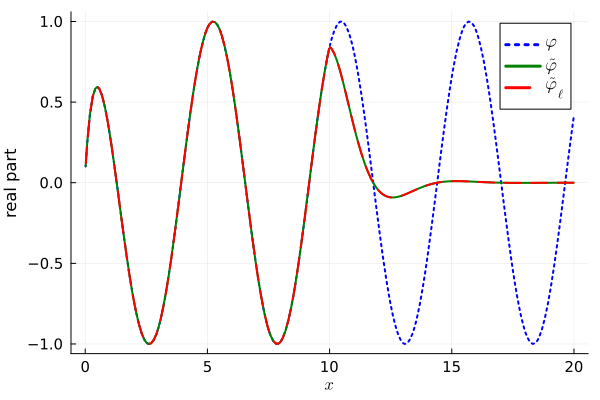
\includegraphics[width=1\textwidth]{wavemaker_modal_solution.pdf}
    \caption{Exact solution $\varphi_{\text{ref}}$, its analytic extension
    $\tvarphi_{\text{ref}}$, and the numerical approximation $\tvarphi_{\ell,h}$. The vertical dashed line indicates the start of the PML layer.}
    \label{fig:wavemaker-comparison-exact-numerical}
  \end{subfigure}\hfill
  \begin{subfigure}[t]{0.49\linewidth}
    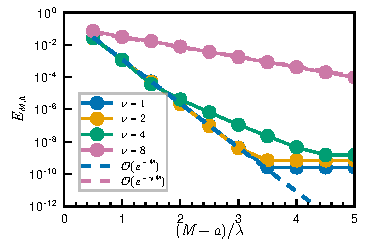
\includegraphics[width=1\textwidth]{convergence_pml_planewave_vary_depth.pdf}
    \caption{Convergence to exact solution as the truncation length $M$ is increased for different values of the parameter $\nu$. The dashed lines are the expected reference slopes.}
    \label{fig:convergence-wavemaker}
  \end{subfigure}
  \caption{Solution to the wave-maker problem (left) and convergence for various values of $\nu$ (right).}
\end{figure}

As observed in~\cref{fig:convergence-wavemaker}, the rate of exponential decay of truncation errors appears to deteriorate as $\nu$ increases. This is easy to understand if we consider the behavior of $k$ and $\gamma_1$ as a function of $\nu$, which is shown in~\cref{fig:propagative-vs-evanescent}. As can be seen (and it easily follows from~\cref{eq:dispersion-relation,eq:disp-evanescent}) we have that $k \to \nu$, $\gamma_1 \to \pi/2$ in the limit $\nu \to \infty$ (in particular $\gamma_1 > k$ for $\nu \gtrapprox 2.3$). As such, the truncation of the evanescent mode becomes dominant for sufficiently large $\nu$, and a large PML layer may be needed to obtain a small truncation error. While not a major drawback of the method for reasonably small values of $\nu$ --- the method still converges exponentially fast for any fixed $\nu$ --- we propose next a possible modification to the PML function~\cref{eq:linear-pml} to improve the truncation errors in the presence of slowly-decaying evanescent modes. 
%
\begin{figure}[ht]
  \centering
  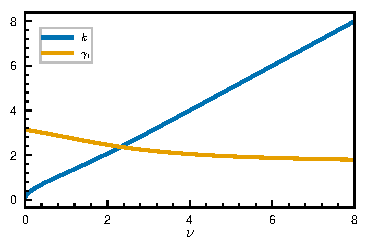
\includegraphics[width=0.5\textwidth]{propagative_vs_evanescent.pdf}  
  \caption{Wavenumber $k$ versus $\gamma_1$ as a
  function of $\nu$.}
  \label{fig:propagative-vs-evanescent}
\end{figure}

Inspired by~\cite{Vial:12}, we modify our complex stretching to account not only for the propagating surface-wave mode but also for the slowest decaying evanescent mode, hence ensuring the effectiveness of the PML for a larger range of $\nu$. The main idea is to employ two different absorbing layers: a complex scaled layer, as before, to absorb the propagating mode, followed by a real stretching to accelerate the convergence of the evanescent mode. In more detail, we replace the PML function~\cref{eq:linear-pml} by:
\begin{align}
    \label{eq:two-layer-pml}
  \tau_{\text{two-layer}}(x_1) &=  
  \begin{cases}
    \tau(x_1), & |x_1| \leq b, \\
    \tau(\nu x_1) - \tau(\nu b) + \tau(b) & |x_1| > b, \\
\end{cases}
\end{align}
where $b > a$ is a new parameter controlling the start of the real-stretching layer. An illustration of this two-layered PML is shown in~\cref{fig:two-layer-pml}. 
% %%%%%%%%%%%%%%%%%%%%%%%%%
% \begin{align}
%     \label{eq:two-layer-pml}
%   \tau(x_1) &=  
%   \begin{cases}
%     \nu x_1 + ic(\nu x_1+a), & x_1 \leq -b, \\
%     x_1 + ic (x_1+a), & -b \leq x_1 \leq -a, \\
%     x_1, & |x_1| < a, \\
%     x_1 + i c (x_1 - a) & a \leq x_1 \leq b,\\
%     \nu x_1 + i c (\nu x_1 - a) & x_1 \geq a,
% \end{cases}
% \end{align}
% %%%%%%%%%%%%%%%%%%%%%%%%%
%%%%%%%%%%%%%%%%%%%%%%%%%
It is important to note that the real stretching increases the frequency of the oscillatory mode, and therefore should only be applied \emph{after} the complex stretching layer.
% Next, we describe a simple rationale used to PML layer into the first complex scaling layer and the real stretching layer.

Given the start of the PML layer $a$, and the truncation parameter $M$, we chose $b$ by the following simple rationale. Supposing the propagating mode decays by $\e^{-ck(b-a)}$, while the evanescent mode decays by $\e^{-\gamma_1 \nu (M-b)}$, requiring both errors to be equal yields
\begin{align}
 b = \frac{cka + \gamma_1 \nu M}{ck+\gamma_1 \nu},
\end{align} 
which provides a way for choosing $b$ given the other problem parameters. Inserting this expression into the decay rate of the propagating mode, $\e^{-ck(b-a)}$, gives:
\begin{equation}
    \e^{-ck(b-a)} \sim \mathcal{O}(e^{-ck \mu M}), \quad \mbox{where} \quad \mu = \frac{\gamma_1 \nu}{ck + \gamma_1 \nu}.
    \label{eq:two-layer-decay}
\end{equation}
\Cref{eq:two-layer-decay} provides the expected decay rate of the $\tvarphi$ when the two-layer PML function~\cref{eq:two-layer-pml} is used. The constant $\mu < 1$ in~\cref{eq:two-layer-decay} provides an idea of the deterioration compared~\cref{eq:decay-rate} for the cases where $ck < \gamma_1$ (i.e. cases for which the decay is dominated by the propagating mode). Importantly, as $\nu \to \infty$, we have $\mu \to \pi / (2c + \pi)$, meaning the decay rate is at worst a constant factor slower than $\e^{-ck\mu}$; for $c = 1$, for example we have $\mu \approx 0.61$ as $\nu \to \infty$. As can be seen in~\cref{fig:convergence-stretching-vary-depth}, the proposed idea significantly improves the truncation error, even for values of $\nu$ as large as $32$. Furthermore, we observe that as $\nu$ increases the decay appears to match the the expected asymptote of $\mathcal{O}(\e^{-k \pi/(\pi+2)M})$, shown as a dashed line in~\cref{fig:convergence-stretching-vary-depth}. 
%
\begin{figure}[ht]
  \centering
  \begin{subfigure}{0.49\linewidth}
    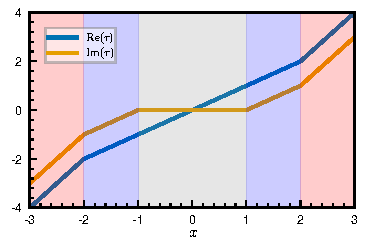
\includegraphics[width=\textwidth]{pml_real_and_imag.pdf}
    \caption{Two-layered PML with $a=1$, $b=2$, $c=1$, $\nu=2$}
    \label{fig:two-layer-pml}
  \end{subfigure}\hfill
  \begin{subfigure}{0.49\linewidth}
    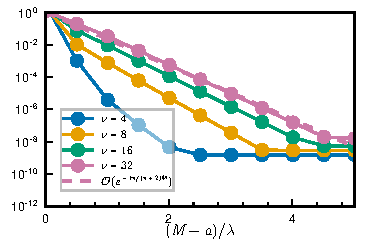
\includegraphics[width=1\textwidth]{convergence_pml_stretch_planewave_vary_depth.pdf}
    \caption{Convergence for large values of $\nu$ with two-layer PML.}
    \label{fig:convergence-stretching-vary-depth}
  \end{subfigure}
  \label{fig:convergence-modal-solution}
  \caption{Two-layered PML function (left) and its convergence properties (right)}
\end{figure}

Although not the main focus of this paper, we present in~\cref{fig:mesh-convergence} convergence results with respect to the mesh refinement. As explained
in~\cref{sec:discretization-error}, we use a composite quadrature rule to
discretize the domain, which in our code is represented by an explicit
parametrisation. After splitting the domain into elements of approximate size $h$, we use a $P$-point
Gauss-Legendre quadrature rule per element; such a quadrature rule exactly
integrates polynomials of order up to $2n-1$, and the Gauss-Legendre
nodes can be used to interpolate a polynomial of order $n-1$. Following~\cref{sec:discretization-error}, we expect a convergence of order $P+1$ for smooth surfaces, and of order $P$ for surfaces with a corner (assuming of course that the solution we seek to approximate is sufficiently regular). This is precisely what is observed for the wavemaker problem in~\cref{fig:mesh-convergence}, where a convergence of order $P$ appears to be recovered. (For this example we took a PML of length $4 \lambda$, where $\lambda$ is the wavelength, which was enough to ensure sufficiently small truncation errors.)

\begin{figure}
  \centering
  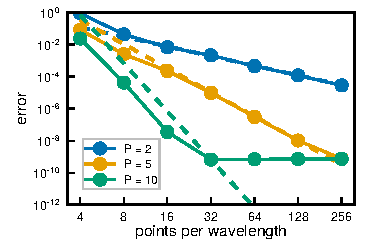
\includegraphics[width=0.5\textwidth]{mesh_convergence_waveguide.pdf}
  \caption{Convergence to the modal solution for $\nu=2$ as the number of
  points per wavelength is increased for three different $P$-point
  Gauss-Legendre quadratures. The expected convergence rate of order $P$
  described in~\cref{sec:discretization-error}, shown as dashed lines of the same color, is recovered.}
  \label{fig:mesh-convergence}
\end{figure}

\subsection{Scattering problem}

Having validated the proposed algorithm and its implementation in the
previous sections, we focus now on the classical scattering problem. In the following examples, we consider an incident field, corresponding to a right-going propagating mode, given by 
\begin{align}
  \varphi^{inc}(x_1,x_2) = \frac{\cosh(k(x_2+1))}{\cosh(k)} e^{i k x_1}.
\end{align}
Writing the total field as
\begin{align}
  \varphi^{tot} = \varphi^{inc} + \varphi,
\end{align}
we seek to find a scattered field $\varphi$ satisfying the radiation condition~\cref{eq:radiation-condition}. It follows from the problem linearity that $\varphi$
satisfies~\cref{eq:water-waves-system} with $f_1 = 0$ and $f_2 = -\nabla \phi
\cdot \bn$; i.e. $\varphi$ satisfies the following boundary condition:
\begin{align}
  \varphi = - \nabla \varphi^{inc} \cdot \bn, \quad \bx \in \Gamma_o \cup \Gamma_b
\end{align}
We consider next three different geometries for the scattering problem: (i) some fully submerged jellyfish-like obstacles in a variable topography, (ii) a wave-guide with two piercing obstacles, and (iii) a topography containing a step profile. 

\subsubsection{Submerged obstacles}

For this geometry, we take a bottom topography given by the following height function:
\begin{align}
    \mathrm{topography}(s) = (s,-1 + \e^{-s^2/4} \sin(2\pi s /\lambda).)
\end{align}
This yields a ``bump-like'' perturbation to a constant depth\footnote{Although this is not compact perturbation to a constant depth, the exponential decay of the depth function towards $1$ behaves very similarly, and is easier to construct than a compact and $C^\infty$ perturbation.}. In addition to the bump-like topography, we add three jellyfish-like obstacles given by the following parametrization (after appropriate rotation, translation, and scaling):
\begin{align}
    \mathrm{jellyfish}(s) = (r(s)\cos(s),r(s)\sin(s)) \quad \mbox{where} \quad r(s) = 1+0.3\cos(4s+2\sin(s))
\end{align}
The resulting geometry, as well as the scattered field, can be viewed in~\cref{fig:jellyfish-fields}, where we display the incident, total, and scattered fields for a value of $\nu=4$ (which yields a wavelength $\lambda \approx 1.57$). We used a one-wavelength PML layer of strength $c=1$ starting at $a=3\lambda$ (the dashed vertical line). The damping of the scattered field inside the PML-layer is clearly visible in~\cref{fig:jellyfish-fields} (bottom), especially for $x_1 > 2\lambda$. The main effect of the topography and obstacles is to cause a phase shift in the transmitted wave, as can be observed by comparing the incident field (top) to the total field (center) in~\cref{fig:jellyfish-fields}. In this example, we used a mesh of size $\lambda/30$, and a value of $P=5$. 

\begin{figure}[ht!]
  \centering
  \vspace{-30pt}
  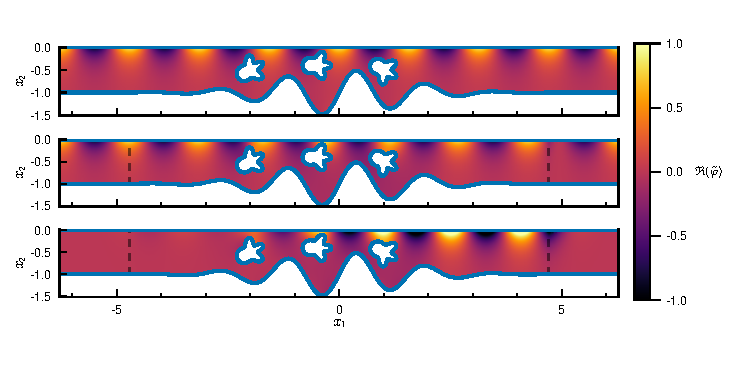
\includegraphics[width=1\textwidth]{jellyfish_fields.pdf}
  \vspace{-30pt}
  \caption{Incident field (top), total field (middle), and scattered field (bottom) for three jellyfish-like over a variable topography. The dashed lines indicate the start of the PML layer, after which we observe a decay of the scattered field (bottom) due to the complex stretching.}
  \label{fig:jellyfish-fields}
\end{figure}

Since no exact solution is known for this scattering problem, we performed instead a self-convergence test, where we evaluated $\varphi$ on a uniform mesh of the rectangle $[1.5\lambda,2.5\lambda] \times [-0.75 \times -0.25] \subset \Omega$, and compared the results to a reference solution obtained using $256$ points-per-wavelength. We fixed $P=5$, as in the previous example, as in the previous example, and varied the number of points per wavelength from $4$ to $128$. Since the geometry is smooth, we expect from~\cref{sec:discretization-error} a convergence of order of $P+1 = 6$, which appears to agree with the convergence rate observed in~\cref{fig:convergence-jellyfish}. 
\begin{figure}[ht!]
  \centering
  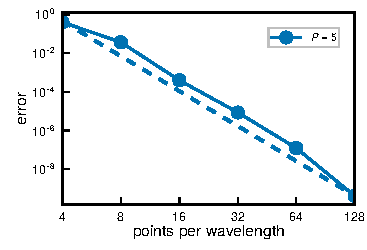
\includegraphics[width=0.5\textwidth]{mesh_convergence_jellyfish.pdf}
  \caption{Self-convergence of scattering problem for the geometry shown in~\cref{fig:scattered-field-submerged}. A reference solution with $256$ points-per-wavelength was used when computing the error. The reference dashed-like shows the expected convergence order of $h^{-6}$. }
  \label{fig:convergence-jellyfish}
\end{figure}

\subsubsection{Piercing obstacles}\label{sec:piercing-geo}

While we have insofar considered only fully submerged obstacles (i.e. the free-surface coincides with $\R \times \{0\}$), piercing objects can be handled in a similar fashion. From an application point of view, piercing obstacles are particularly interesting since many objects of interest (ships, docks, buoys) are usually found at the free surface. For simplicity, we take here a geometry given by two piercing semi-circles of radius $r=1/4$ centered at $x_1 = \pm x_c$, with $x_c = r + 1/2$. This geometry creates a free-surface with three disconnected components: $[-\infty, -1] \times \left\{0 \right\} \cup [-0.5,0.5] \times \left\{0 \right\} \cup [0.5, \infty] \times \left\{0 \right\}$. 

In~\cref{fig:piercing-field} we display both the aforementioned geometry, as well as the scattered field for a value of $\nu=4$. Unlike the submerged obstacle, we observe a significant scattered field both before (on the left) and after (on the right) of the obstacles (see the supplementary material for an animation of the total field). Again, as expected, the scattered field decays after the PML. 
%
\begin{figure}
  \centering
  \vspace{-50pt}
  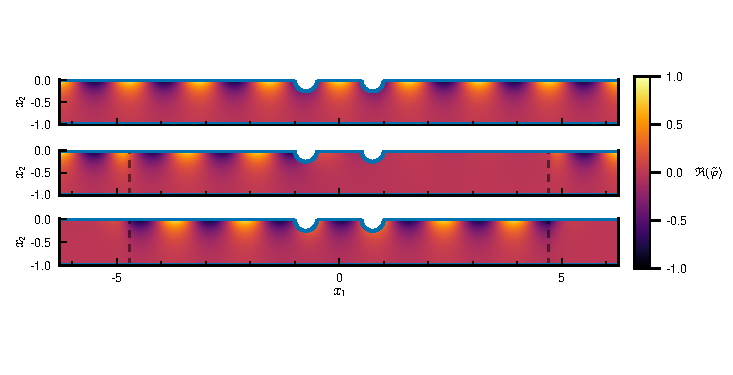
\includegraphics[width=1\textwidth]{double_piercing_fields.pdf}
  \vspace{-50pt}
  \caption{Incident (top), total (middle), and scattered (bottom) fields in the presence of two piercing bodies.}
  \label{fig:piercing-fields}
\end{figure}
%
The convergence with respect to mesh refinement is shown in~\cref{fig:piercing-convergence}, where the reference line has a slope of $P=5$. 
\begin{figure}
  \centering
  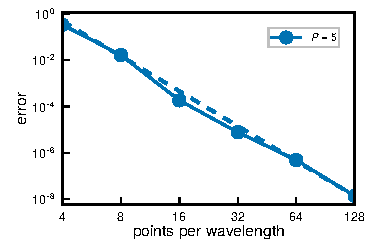
\includegraphics[width=0.5\textwidth]{mesh_convergence_double_piercing.pdf}
  \caption{Convergence in the presence of piercing body.}
  \label{fig:piercing-convergence}
\end{figure}

We will revisit this geometry again when looking at resonant frequencies in~\cref{sec:resonant-freq}. 

\subsubsection{Step topography}

The final geometry considered for the scattering problem is that of a topography with a different depth as $x_1 \to \pm \infty$. In particular, we consider the smooth step-like topography given by
\begin{align}
    \textrm{step}(s) = -1 + \Delta d (1+\tanh(5s))/2,
\end{align}
where for this particular example we took $\Delta d = 0.75$, so that the shallow region has a depth of $1/4$.~\Cref{fig:step-fields} shows the scattered field for $\nu=4$, where once again the decay of $\tvarphi$ inside the PML layer becomes apparent. 
\begin{figure}[ht!]
  \centering
  \vspace{-40pt}
  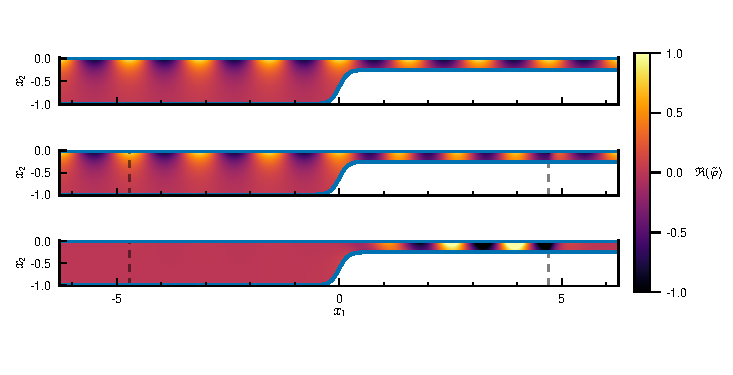
\includegraphics[width=1\textwidth]{step_fields.pdf}
  \vspace{-40pt}
  \caption{Scattered field for step-like geometry.}
  \label{fig:step-fields}
\end{figure}
In~\cref{fig:step-fields} we plot the incident field (which, we recall, does not vanish on the topography) as well as the total field. The change in the wavelength is clearly visible on the right of the step, where the effective frequency is increased. 

\subsection{Resonant frequencies}\label{sec:resonant-freq}

In this final set of examples, we consider the challenging problem of finding resonant frequencies to the water-waves problem. More precisely, we seek to find the values of the impedance $\nu$ such that~\cref{eq:water-waves-system} has a nontrivial solution for $f_1=f_2=0$. Using the boundary integral formulation~\cref{eq:BIE-long}, this corresponds to finding eigenvalues $\nu$ and eigenfunctions $\tvarphi_\nu$ solving the following (generalized) linear eigenvalue problem:
%
\begin{align}
  \label{eq:BIE-eigenvalue}
  -\frac{\tvarphi_\nu(\bx)}{2} + D_{\Gamma}[\tvarphi_\nu](\bx) =  -\nu S_{\Gamma_f}\left[\tau'\tvarphi_\nu\right](\bx), \quad \bx \in \Gamma.
\end{align}
%

To show what a typical spectrum looks like, we solve a discrete version of~\cref{eq:BIE-eigenvalue} for the piercing geometry of~\cref{sec:piercing-geo}. The full set of eigenvalues is shown in \Cref{fig:double-piercing-spectrum}. We comment on a few interesting features of~\cref{fig:double-piercing-spectrum}. First, part of the spectrum appears to follow a straight line of slope $\approx -1$. These eigenvalues correspond to the continuous spectrum of the original problem, given by $\R^+$, which is deformed by the PML. Second, there is a bifurcation point, which is similar to what was observed in~\cref{?}. Third, there are a set of ``isolated'' eigenvalues with a small negative part, that appear at a approximately regular intervals. These last eigenvalues are localized near the obstacle, and do not change significantly as the PML function $\tau$ is modified. We plot in ~\cref{fig:double-piercing-eigenfunction} one of these localized eigenfunctions, corresponding to the red eigenvalue in~\cref{fig:double-piercing-spectrum}. 
\begin{figure}[ht!]
  \centering
  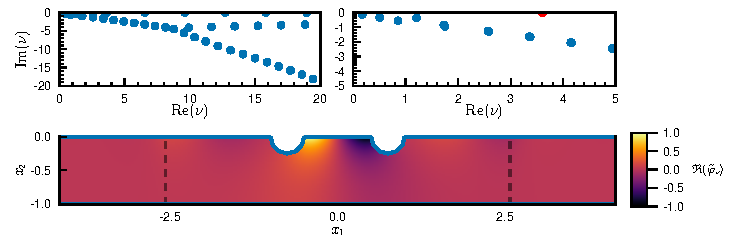
\includegraphics[width=1\textwidth]{eigenvalue_problem.pdf}
  \vspace{-20pt}
  \caption{Complex resonances of piercing geometry with two semi-circles. To top figures show the spectrum, while the bottom shows an eigenfunction for the eigenvalue in red in the top-right figure.}
  \label{fig:double-piercing-spectrum}
\end{figure}


% \subsubsection{Resonant frequencies}
% % \begin{figure}
% %   \centering
% %   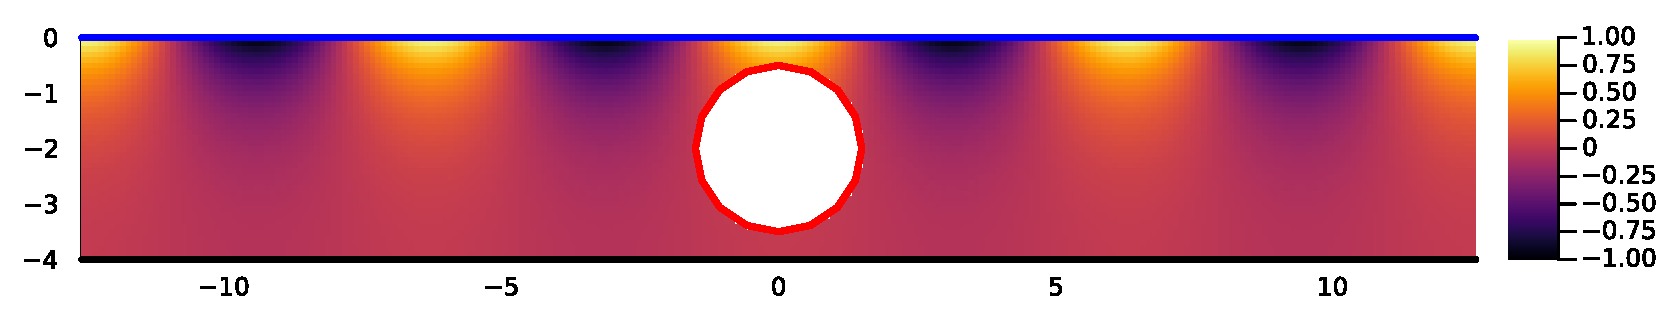
\includegraphics[width=0.95\textwidth]{inc_field_contour_depth_4.pdf}\\
% %   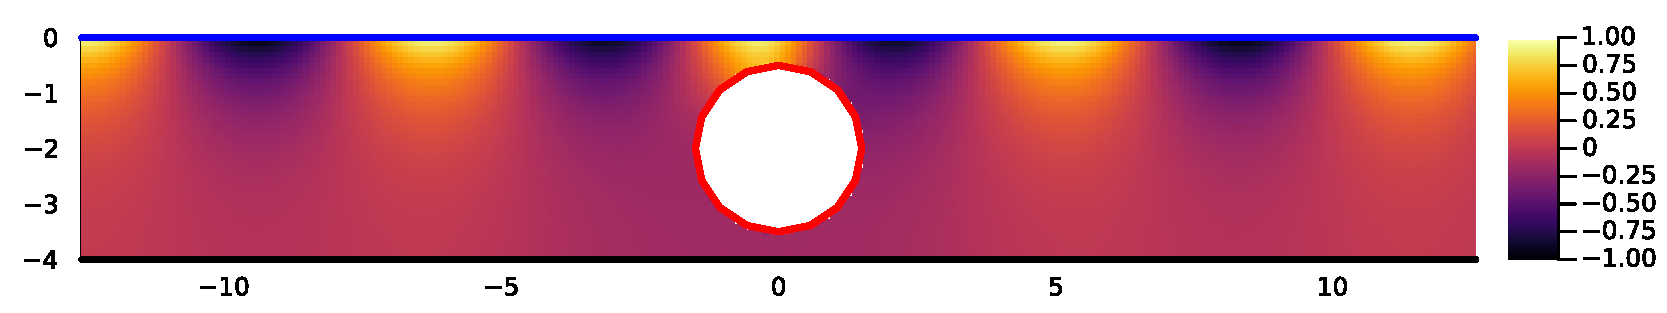
\includegraphics[width=0.95\textwidth]{total_field_contour_depth_4.pdf}
% %   \caption{Incident and total field for scattering problem. A phase-shift is observed after the obstacle.}
% %   \label{fig:total-incident-submerged-contour}
% % \end{figure}

% \subsection{Resonance modes}

% \begin{figure}
%   \centering
%   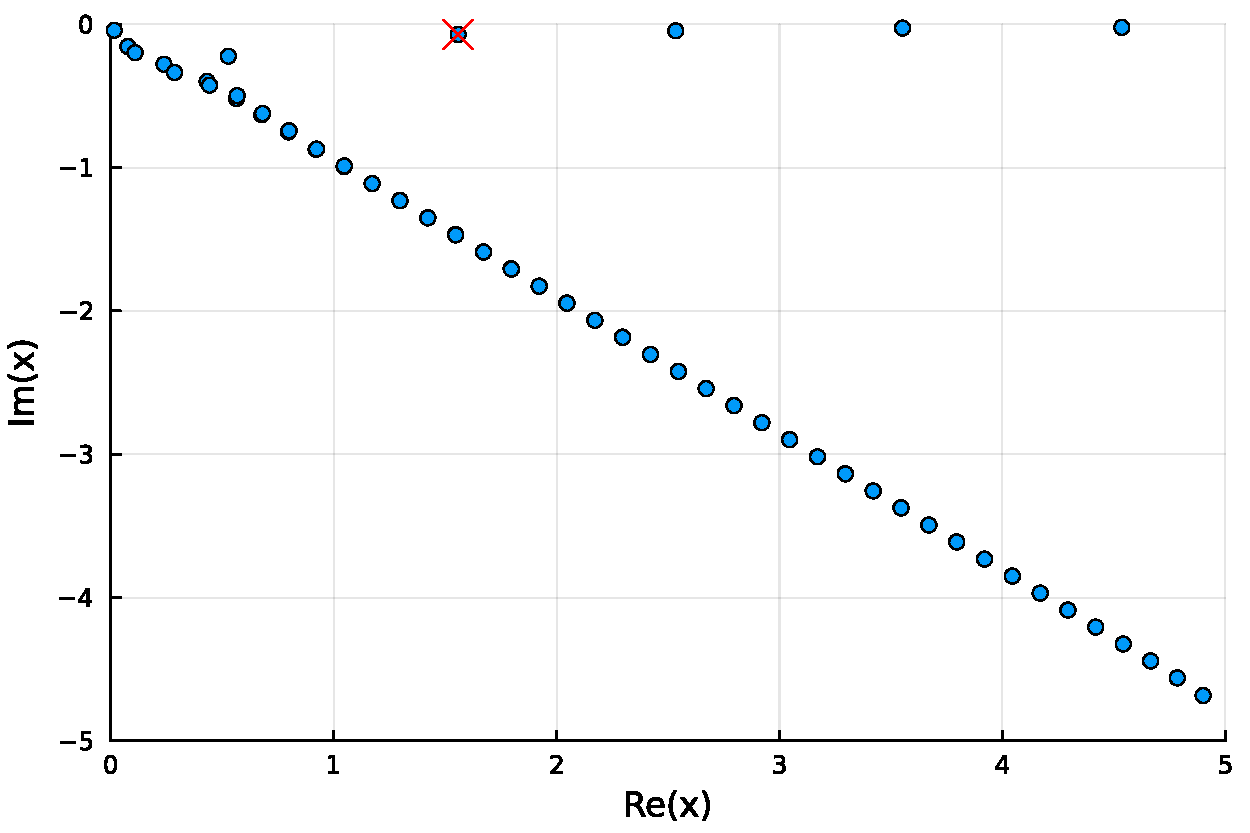
\includegraphics[width=0.5\textwidth]{eigenvalues_two_piercing_depth_4.pdf}
%   \caption{Eigenvalues associated with the two piercing semi-circles show
%   in~\cref{fig:scattered-two-piercing-contour}. The red cross shows an example
%   of a nearly resonant eigenvalue $\lambda$ with $\Re(\lambda) \approx 1.56$ and
%  $\Im(\lambda) \approx - 0.07$}
%   \label{fig:eigenvalues}
% \end{figure}

% \begin{figure}
%   \centering
%   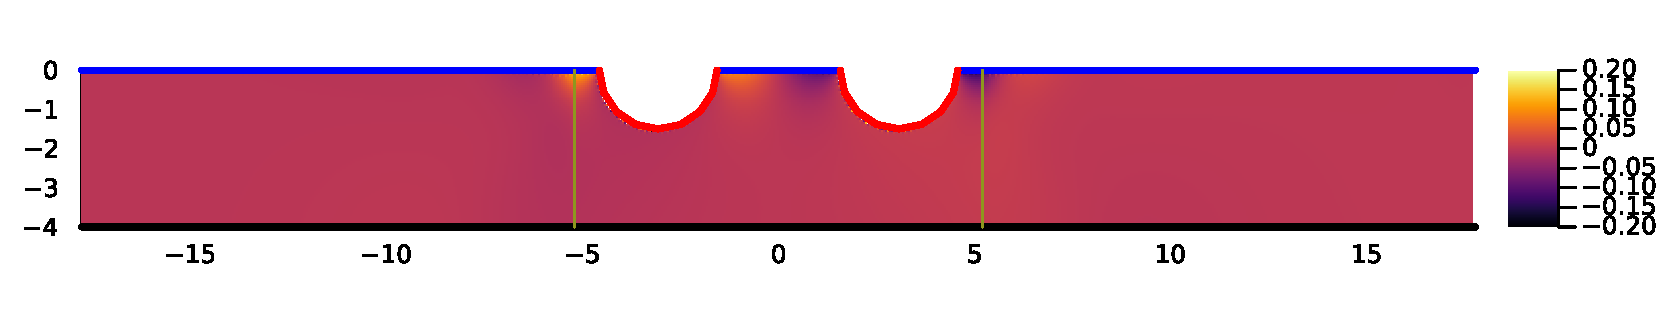
\includegraphics[width=0.95\textwidth]{eigenfunction_two_piercing_depth_4.pdf}
%   \caption{Eigenfunction associated with eigenvalue}
%   \label{fig:eigenfunction}
% \end{figure}

% \subsection{Non-orthogonal PMLs}\label{sec:nonorthogonal-pml}

\section{Open theoretical problems}
This work has opened up several challenging theoretical questions that were not addressed in this paper. 

The logarithmic growth of the single-layer kernel makes it difficult to pose a functional framework for analyzing the well-posedness of~\cref{eq:BIE} in the usual Sobolev spaces. 
% It is easy to see, for instance, that for large values of $\bx$ the right-hand-side of~\cref{eq:BIE} behaves as 
% \begin{align}
%     \log(|\tau(\bx)|) \int_{\Gamma_f} f_1(\by) \de s(\by) + \int_{\Gamma_n} f_2(\by) \de s(\by)
% \end{align}
% This logarithmic growth has to be balanced by a similar logarithmic growth on the left-hand side. 
A possible way to circumvent such theoretical difficulties is to consider instead a Green's function $\widetilde{G}^D$ satisfying a (homogeneous) Dirichlet boundary condition at $x_2 = H$ for some $H>0$~\cite{preston2008integral}. By the method of images, we have that $\widetilde{G}^D$ is given by
\begin{align}
    \label{eq:dirichlet-green-function}
    \widetilde{G}^D(\bx,\by) = &-\frac{1}{4\pi}\log \left((\tau(x_1) - \tau(y_1))^2 + (x_2 - y_2)^2\right) \\
    &- \frac{1}{4\pi}\log \left((\tau(x_1) - \tau(y_1))^2 + (x_2 - y_2^r)^2 \right) \nonumber
\end{align}
where $y_2^r = 2H - y_2$ is the image point. With this Dirichlet Green's function, one obtains a linear decay of the single-layer kernel as $|\by| \to \infty$, which in turn may help define an appropriate functional framework for equations like~\cref{eq:BIE}. 

On the other hand, to investigate the equivalence between the boundary integral equation~\cref{eq:BIE} and the complex-scaled water-waves problem~\cref{eq:water-waves-system-pml}, consider a   density $\sigma : \Gamma \to \C$ solution of $\cref{eq:BIE}$, and define the function $\tvarphi: \Omega \to \C$ by
\begin{align}
\label{eq:tentative-solution}
\tvarphi(\br) = \mathcal{D}_{\Gamma}[\sigma](\br) - \mathcal{S}_{\Gamma}[f - \alpha \tau' \sigma](\br).
\end{align}
One would like to show that~\cref{eq:tentative-solution} is a solution to the original problem~\cref{eq:water-waves-system-pml}. The fact that~\cref{eq:tentative-solution} satisfies the PDE~\cref{eq:pml-laplace-real} follows directly from the choice of the integral representation. This means that we may write
\begin{align}
\label{eq:tentative-solution-representation-formula}
\tvarphi(\br) = \mathcal{D}_{\Gamma}[\tvarphi](\br) - \mathcal{S}_{\Gamma}[\tau' \nabla \tvarphi \cdot \bn](\br).
\end{align}
Taking the Dirichlet trace of~\cref{eq:tentative-solution} and using the fact that $\sigma$ solves~\cref{eq:BIE} we obtain that $\tvarphi = \sigma$ on $\Gamma$. Subtracting~\cref{eq:tentative-solution-representation-formula} from~\cref{eq:tentative-solution} yields
\begin{align}
\label{eq:zero-potential}
\mathcal{S}_{\Gamma}[\tau' \nabla \tvarphi \cdot \bn - f + \tau'\alpha \tvarphi](\br) = 0, \quad \br \in \Omega.
\end{align}
Equality \cref{eq:zero-potential} can be extended to $\Gamma$ to give:
\begin{align}   
\label{eq:tentative-solution-representation-formu}
S_{\Gamma}[\tau' \nabla \tvarphi \cdot \bn - f + \tau'\alpha \tvarphi](\bx) = 0, \quad \bx \in \Gamma.
\end{align}
As a consequence, $\tvarphi$ as given by~\cref{eq:tentative-solution} solves the water-waves system~\cref{eq:water-waves-system-pml} if the single-layer operator $S_\Gamma$ is ``injective" in a certain sense. However, due to the current limited understanding of the mapping properties of the single-layer operator in this scenario, we are unable to provide a more precise analysis at this time.

\begin{remark}[Neumann Green's function]
While the use of a Dirichlet Green's was motivated above for theoretical reasons, the use of a Green's function satisfying a Neumann boundary condition at a flat bottom $x_2 = -1$ is more advantageous from a numerical point of view, for in that case only the perturbations to the constant depth topography need to be discretized when $\Gamma \cap \R \times \{ x_2<-1 \}  = \emptyset$ (meaning $\Omega$ lies above the $x_2=-1$ line). Such a Green's function is easy to construct once again by the method of images
\begin{align}
    \label{neumann-green-function}
    \widetilde{G}^N(\bx,\by) = &-\frac{1}{4\pi}\log \left((\tau(x_1) - \tau(y_1))^2 + (x_2 - y_2)^2\right) \\
    &- \frac{1}{4\pi}\log \left((\tau(x_1) - \tau(y_1))^2 + (x_2 - y_2^d)^2 \right) \nonumber
\end{align}
where $y_2^d = 2 - y_2$. Unlike the Dirichlet Green's function, however, $\widetilde{G}^N$ still possesses a logarithmic growth at infinity. In this paper, we opt for simplicity and utilize the free-space Green's function $\widetilde{G}$ in all of the numerical examples of~\Cref{sec:numerical-results}. As it turns out, the numerical solutions we find decay exponentially fast as the truncation parameter is increased, even for the free-space Green's function which grows logarithmically. To our knowledge, a rigorous framework for understanding solutions of~\cref{eq:BIE} when $\widetilde{G}$ is used (which grows at infinity) is an open question. 
\end{remark}

\section{Conclusions}\label{sec:conclusions} In this paper, we presented a novel boundary integral formulation for solving the two-dimensional finite depth water waves problem. While our numerical results are promising, there is still much theory to be developed to better understand the truncation errors. Future directions of research that we find interesting are extensions to infinite depth and the three-dimensional problem. 

\appendix

\section{Complex-scaled fundamental solution}\label{sec:fundamental-solution}
Let $x_1\in\R\mapsto \tau(x_1)\in\C$ be as in section \ref{sec:complex-stretching} a   continuous and piecewise continuously differentiable function satisfying \eqref{eq:tau-condition-real}. 
 In this section, we provide a direct proof that $$\widetilde{G}(\bx,\by)=G(\btau(\bx),\btau(\by))\mbox{ where }\btau(\bx)=(\tau(x_1),x_2)$$  is the free-space fundamental solution of the complex-scaled Laplace equation,  i.e. that $\widetilde{G}$
 satisfies 
 \begin{align}
 \label{eq:identityGreen}
  \int_{\R^2} \nabla_\by\widetilde{G}(\bx,\by) \cdot   A(\by) \nabla v(\by)   \de \by = v(\bx),\quad \forall \bx\in \R^2,
 \end{align}
 for all test functions $v \in \mathcal{D}(\R^2)$, where $A$ is given by \eqref{eq:water-waves-system-pml}.
 %$$A(\by)=\begin{bmatrix}
 %    \tau'(y_1)^{-1} & 0\\
  %  0 & \tau'(y_1)
 %\end{bmatrix}$$
 %$A(\by)= \det(J(\by))J(\by)^{-1}(J(\by)^{-1})^t$ and  $J(\by)$ is the Jacobian matrix of the application $\by\mapsto \btau(\by)$, supposed to be continuous and piecewise continuously differentiable. 
 
By continuity arguments, it suffices to prove \eqref{eq:identityGreen} for points $\bx$ where $\btau$ is differentiable, and let us denote by $I(\bx)$ the left hand side of \eqref{eq:identityGreen}. Note that  $\widetilde{G}(\bx,\by)$ is well-defined for all $\bx$, $\by$ in $\R^2$, as soon as $\bx\neq\by$. Indeed, suppose that 
$$(\tau(x_1)-\tau(y_1))^2+(x_2-y_2)^2=0,$$
then 
$$\real (\tau(x_1)-\tau(y_1))=0,$$
which implies by \eqref{eq:tau-condition-real} that $x_1=y_1$, and finally that $\bx=\by$. 
Now by the
 properties of the Lebesgue integral and the symmetry of $A(\by)$, it holds that
 $$I(x)=\lim_{\varepsilon\to 0}\int_{|\by-\bx|>\varepsilon}  A(\by)\nabla_\by\widetilde{G}(\bx,\by) \cdot  \nabla v(\by)    \de \by.$$
 Integrating by parts and using that 
 $$\nabla_{\by} \cdot( A({\by}) \nabla_\by\widetilde{G}(\bx,\by))=0\mbox{ if }\by\neq \bx,$$
 we obtain that
 $$I(\bx)=\lim_{\varepsilon\to 0}\frac{1}{\varepsilon}\int_{|\by-\bx|=\varepsilon}A({\by}) \nabla_\by\widetilde{G}(\bx,\by)\cdot (\bx-\by)v(\by)    \de s_\by.$$
 On the other hand, the chain rule and the definition of the function $G$ lead to 
 %$$\nabla_\by\widetilde{G}(\bx,\by)=\frac{J(\by)^t(\btau(\bx)-\btau(\by))}{2\pi(\btau(\bx)-\btau(\by))\cdot(\btau(\bx)-\btau(\by)) },$$
 $$\nabla_\by\widetilde{G}(\bx,\by)=\frac{1}{2\pi }\frac{1}{(\tau(x_1)-\tau(y_1))^2+(x_2-y_2)^2}\begin{bmatrix}
  \tau'(y_1)(\tau(x_1)-\tau(y_1))  \\
    x_2-y_2 
 \end{bmatrix},$$
 so that by definition of $A(\by)$:
  %$$I(\bx)=\lim_{\varepsilon\to 0}\frac{1}{2\pi\varepsilon}\int_{|\by-\bx|=\varepsilon}\det(J(\by))\frac{J(\by)^{-1}(\btau(\bx)-\btau(\by))\cdot (\bx-\by)}{(\btau(\bx)-\btau(\by))\cdot(\btau(\bx)-\btau(\by)) }v(\by)  \de s_\by.$$
  $$I(\bx)=\lim_{\varepsilon\to 0}\frac{1}{2\pi\varepsilon}\int_{|\by-\bx|=\varepsilon}\tau'(y_1)\frac{ \tau'(y_1)^{-1}(\tau(x_1)-\tau(y_1))(x_1-y_1) +(x_2-y_2)^2}{(\tau(x_1)-\tau(y_1))^2+(x_2-y_2)^2}v(\by)  \de s_\by.$$
  Now parametrizing the circle by $\by = \bx + \epsilon\br(\theta)$, with
 $\br(\theta) = (\cos(\theta),\sin(\theta))$ and using straightforward Taylor expansions, this leads to 
 %$$I(\bx)=v(\bx)\det(J(\bx))\int_0^{2\pi} \frac{1}{\br^t(\theta) J^t(\bx) J(\bx) \br(\theta)} \de \theta.$$
 $$I(\bx)=\frac{v(\bx)}{2\pi}\int_0^{2\pi} \frac{\tau'(x_1)}{\tau'(x_1)^2\cos(\theta)^2+\sin(\theta)^2} \de \theta.$$
We conclude by using the following classical result of complex analysis: 
$$\int_0^{2\pi} \frac{1}{\alpha^2\cos(\theta)^2+\sin(\theta)^2} \de \theta=\frac{2\pi}{\alpha}$$
which holds for all $\alpha\in\C$ such that $\real(\alpha)>0$. The result can be proved first for real $\alpha$, rewriting the identity as
$$\imag \left(\int_{\mathcal C}\frac{dz}{z}\right)=2\pi$$
where ${\mathcal C}$ is an ellpise defined by  ${\mathcal C}=\{\alpha\cos(\theta)+i\sin(\theta); 0\leq\theta\leq 2\pi\}$. Then one concludes that the identity still holds for complex $\alpha$ by analyticity. 

\section{Mesh convergence}

% Letting $J = [a b; c d]$, we can compute


% We now investigate the asymptotic behavior of $\widetilde{R}(\bx,\by) =
% R(\tau(\bx),\tau(\by))$ as $\by \to \bx$. First, we may write $\tau(\bx) -
% \tau(\by) = J(\bx)(\bx - \by) + \mathcal{O}(|\bx - \by|^2)$, so that
% \begin{align}
%   \widetilde{R}^2(\bx,\by) &= (\tau(\bx) - \tau(\by)) \cdot (\tau(\bx) - \tau(\by)) + \mathcal{O}(R^4)\\
%               &= (\bx-\by)^t J(\bx)^t J(\bx) (\bx-\by) + \mathcal{O}(R^4)
% \end{align}
% This show in particular that, provided the eigenvalues of $J^tJ$ are s.t.
% $ 0< c < \lambda < C < \infty$, then $\widetilde{R}$ goes to zero at the same rate
% as $R$.

% Finally, we will need the leading order term in the gradient of $\widetilde{R}$. It
% is easier to use $\nabla(\widetilde{R}\cdot\widetilde{R}) = 2\widetilde{R} \nabla\widetilde{R}$
% so that we have
% \begin{align}
%   \nabla(\widetilde{R}\cdot\widetilde{R}) = \nabla((\bx - \by)^t J^t J (\bx - \by)) = 2 J^t J (\bx - \by) + \mathcal{O}(|\bx - \by|^2)
% \end{align}
% We are now ready to show the result.

% %
% First, take a test function $v \in \mathcal{D}(\Omega)$ and multiply and integrate:
% \begin{align}
%   \int_{\Omega} v(\bx) \left(\nabla \cdot \left( \frac{1}{|J^{-1}|}J^{-1}(J^{-1})^t \nabla \widetilde{G}(\bx,\by) \right) + \frac{1}{|J^{-1}|}k^2\widetilde{G}(\bx,\by)\right) \de \bx = v(\by)
% \end{align}
% Split the integral as $\int_\Omega = \int_{\Omega \setminus B_\epsilon(\bx)} + \int_{B_\epsilon(\bx)}$. Consider first the
% non-singular part:
% \begin{align}
%   I_1 = \int_{\Omega \setminus B_\epsilon(\bx)} v(\bx) \left(\nabla \cdot \left( \frac{1}{|J^{-1}|}J^{-1}(J^{-1})^t \nabla \widetilde{G}(\bx,\by) \right) + \frac{1}{|J^{-1}|}k^2\widetilde{G}(\bx,\by)\right) \de \bx
% \end{align}
% Noticing that the operator is in fact $|J|\widetilde{\Delta}$, it follows by
% analyticity of $G$ (not clear to me) that $\widetilde{\Delta} \widetilde{G} + k^2
% \widetilde{G} = 0$ for $\bx \neq \by$, and so $I_1 = 0$. Next we compute $I_2$.
% First note that the second term is has an integrable kernel, so it tends to zero as $\epsilon
% \to 0$. Applying the divergence theorem to the first term we obtain:
% \begin{align}
%   I_1 = -\int_{B_\epsilon(\by)} \nabla v(\bx) \cdot \left( \frac{1}{|J^{-1}|}J^{-1}(J^{-1})^t \nabla \widetilde{G}(\bx,\by)\right) \de \bx  +
%   \int_{\partial B_{\epsilon}(\by)} v(\bx) A(\bx) \nabla \widetilde{G}(\bx,\by) \cdot \bn \de s_\bx
% \end{align}
% The first part of $I_1$ is again integrable, so we need only estimate the second
% one. To compute the $\nabla \widetilde{G}$ we use
% \begin{align}
%   \nabla \widetilde{G}(\bx,\by) \sim \nabla \log (\widetilde{R}(\bx,\by)) &= \frac{1}{\widetilde{R}(\bx,\by)}\nabla \widetilde{R}(\bx,\by) \\
%                                                                   &= \frac{1}{\widetilde{R}^2(\bx,\by)}J^t(\bx)J(\bx)(\bx - \by)
% \end{align}
% Replacing this in the formula we get
% \begin{align}
%   I_1 =  \int_{\partial B_{\epsilon}(\by)} v(\bx) |J(\bx)| \frac{1}{(\bx-\by)^t J^t(\bx) J(\bx) (\bx - \by)} (\bx - \by)\cdot \bn \de s_\bx
% \end{align}
% Now parametrize the circle by $\bx = \by + \epsilon\br(\theta)$, with
% $\br(\theta) = (\cos(\theta),\sin(\theta))$, and replace $J(\bx) \approx
% J(\by)$, $\bn = \br$ to obtain
% \begin{align}
%   I_1 =  |J(\by)| v(\by)\int_0^{2\pi} \frac{1}{\br^t(\theta) J^t(\by) J(\by) \br(\theta)} \de \theta
% \end{align}
% The last thing is thus to compute the integral
% \begin{align}
%   \int_0^{2\pi} \frac{1}{\br^t(\theta) J^t(\by) J(\by) \br(\theta)} \de \theta.
% \end{align}

% Letting $J = [a b; c d]$, we can compute


% For the two-dimensional problem, we have that 
% \begin{align}
%   J = \begin{bmatrix}
%     \tau_{1,1} & \tau_{1,2}\\
%     0 & 1
%   \end{bmatrix}
%   ,\quad 
%   J^{-1} = \begin{bmatrix}
%     1/\tau_{1,1} & -\tau_{1,2}/\tau_{1,1}\\
%     0 & 1
%   \end{bmatrix}
% \end{align}
% and so
% \begin{align}
%   A = |J|J^{-1}(J^{-1})^t = 
%   \frac{1}{\tau_{1,1}}
%   \begin{bmatrix}
%     1 + \tau_{1,2}^2 & -\tau_{1,2}\tau_{1,1} \\
%     -\tau_{1,2}\tau_{1,1} & \tau_{1,1}^2
%   \end{bmatrix}
% \end{align}
% Assuming $\tau_{1,2}$ is purely imaginary, we have that
% \begin{align}
%   \mathrm{Re}(A) = 
%   \begin{bmatrix}
%     \mathrm{Re}\left(\frac{1 + \tau_{1,2}^2}{\tau_{1,1}}\right) & 0 \\
%     0 & \mathrm{Re}(\tau_{1,1})
%   \end{bmatrix}
% \end{align}
% Considering a change of variables of the form $\tau_i = x_i + i\sigma_i(\bx)$,
% we arrive at the following simple condition:
% \begin{align}
%   |\sigma_{1,2}| < 1
% \end{align}


% While in \cref{sec:orthogonal-pml} we considered the special case where
% $\tau(\bx) = (\tau_1(x_1),\tau_2(x_2))$, we present now the generic case with
% $\tau(\bx) = (\tau_1(\bx),\tau_2(\bx))$. The matrix $A$ is then given by
% \begin{align}
%   A = \frac{1}{|J|}
%   \begin{bmatrix}
%     \tau_{2,2}^2 + \tau_{1,2}^2 & -\tau_{2,1}\tau_{2,2} - \tau_{1,2}\tau_{1,1} \\
%     -\tau_{2,1}\tau_{2,2} - \tau_{1,2}\tau_{1,1}  & \tau_{1,1}^2 + \tau_{2,1}^2
%   \end{bmatrix},
% \end{align}

% Determining ellipticity of this matrix (i.e. finding conditions on $\tau$ under
% which $\mathrm{Re}(A)$ is positive definite) in the general case is a somewhat
% cumbersome calculation which we deferred to \cref{sec:ellipticity-of-A}. For the
% numerical examples we consider in \cref{sec:numerical-examples}, it suffices to
% focus on the uni-axial (but non-orthogonal) case, where we assume $\tau_2(\bx) =
% x_2$. The matrix $A$ then simplifies to
% \begin{align}
%   A  =   \begin{bmatrix}
%     \frac{1 - \sigma_{1,2}^2}{1 + i\sigma_{1,1}} & -i\sigma_{1,2} \\
%     -i\sigma_{1,2} & 1 + i\sigma_{1,1}
%   \end{bmatrix}, \quad
%                      \mathrm{Re}(A) =   \begin{bmatrix}
%     \frac{1 - \sigma_{1,2}^2}{1+\sigma_{1,1}^2} & 0 \\
%     0 & 1
%   \end{bmatrix},
% \end{align}
% %
% and strong ellipticity is equivalent to the simple condition:
% \begin{align}
%   \label{eq:ellipticity-condition-nonorthogonal}
%   \left| \sigma_{1,2}(\bx) \right| < 1 \quad \mbox{for all} \quad \bx \in \Omega.
% \end{align}

% In order to give a geometric interpretation to this condition, it is useful to
% consider a simple case given by
% \begin{align}
%   \tau_1 =
%   \begin{cases}
%     x_1 + i \beta (x_1 + \frac{1}{\alpha} x_2 + a) \quad &\mbox{for} \quad x_1 < -\frac{1}{\alpha} x_2 - a, \\
%     x_1 \quad &\mbox{for} \quad |x_1| < \frac{1}{\alpha} x_2 + a, \\
%     x_1 + i \beta (x_1 - \frac{1}{\alpha} x_2 - a) \quad &\mbox{for} \quad x_1 > \frac{1}{\alpha} x_2 + a.
%   \end{cases}
% \end{align}
% The parameters $\alpha$ and $a$ determine the region where the PML is applied,
% and the parameter $\beta$ controls the attenuation strength inside the PML layer
% (see \cref{fig:sch-pml}). By taking taking the limit $\alpha \to \infty$, for
% instance, we recover the case of an orthogonal PML discussed in
% \cref{sec:orthogonal-pml}.

% We are interested in the analytic extension of $\varphi$ when it is
% exponentially decaying at infinity. This leads to consider the analytic
% extension of $\varphi$ for $\Re(x_1)>L$  (resp. $\Re(x_1)<-L$) only for
% $\imag(x_1)>0$ (resp. $\imag(x_1)<0$), so that the propagating surface mode becomes
% exponentially decaying at infinity. Letting $\btau : \R^2 \to
% \C^2$ mapping points $\bx$ on the physical domain to $\widetilde{\bx} = \btau(\bx)$.
% Then, assuming that $\tau(\bx)$ is the identity map for $|x_1|<L$, and defining
% $\widetilde{\varphi}(x_1,x_2) = \varphi(\tau(x_1),x_2)$ as the analytic 

\bibliographystyle{abbrv}
\bibliography{references}

\end{document}
